% Options for packages loaded elsewhere
\PassOptionsToPackage{unicode}{hyperref}
\PassOptionsToPackage{hyphens}{url}
%
\documentclass[
]{book}
\usepackage{amsmath,amssymb}
\usepackage{iftex}
\ifPDFTeX
  \usepackage[T1]{fontenc}
  \usepackage[utf8]{inputenc}
  \usepackage{textcomp} % provide euro and other symbols
\else % if luatex or xetex
  \usepackage{unicode-math} % this also loads fontspec
  \defaultfontfeatures{Scale=MatchLowercase}
  \defaultfontfeatures[\rmfamily]{Ligatures=TeX,Scale=1}
\fi
\usepackage{lmodern}
\ifPDFTeX\else
  % xetex/luatex font selection
\fi
% Use upquote if available, for straight quotes in verbatim environments
\IfFileExists{upquote.sty}{\usepackage{upquote}}{}
\IfFileExists{microtype.sty}{% use microtype if available
  \usepackage[]{microtype}
  \UseMicrotypeSet[protrusion]{basicmath} % disable protrusion for tt fonts
}{}
\makeatletter
\@ifundefined{KOMAClassName}{% if non-KOMA class
  \IfFileExists{parskip.sty}{%
    \usepackage{parskip}
  }{% else
    \setlength{\parindent}{0pt}
    \setlength{\parskip}{6pt plus 2pt minus 1pt}}
}{% if KOMA class
  \KOMAoptions{parskip=half}}
\makeatother
\usepackage{xcolor}
\usepackage{color}
\usepackage{fancyvrb}
\newcommand{\VerbBar}{|}
\newcommand{\VERB}{\Verb[commandchars=\\\{\}]}
\DefineVerbatimEnvironment{Highlighting}{Verbatim}{commandchars=\\\{\}}
% Add ',fontsize=\small' for more characters per line
\usepackage{framed}
\definecolor{shadecolor}{RGB}{248,248,248}
\newenvironment{Shaded}{\begin{snugshade}}{\end{snugshade}}
\newcommand{\AlertTok}[1]{\textcolor[rgb]{0.94,0.16,0.16}{#1}}
\newcommand{\AnnotationTok}[1]{\textcolor[rgb]{0.56,0.35,0.01}{\textbf{\textit{#1}}}}
\newcommand{\AttributeTok}[1]{\textcolor[rgb]{0.13,0.29,0.53}{#1}}
\newcommand{\BaseNTok}[1]{\textcolor[rgb]{0.00,0.00,0.81}{#1}}
\newcommand{\BuiltInTok}[1]{#1}
\newcommand{\CharTok}[1]{\textcolor[rgb]{0.31,0.60,0.02}{#1}}
\newcommand{\CommentTok}[1]{\textcolor[rgb]{0.56,0.35,0.01}{\textit{#1}}}
\newcommand{\CommentVarTok}[1]{\textcolor[rgb]{0.56,0.35,0.01}{\textbf{\textit{#1}}}}
\newcommand{\ConstantTok}[1]{\textcolor[rgb]{0.56,0.35,0.01}{#1}}
\newcommand{\ControlFlowTok}[1]{\textcolor[rgb]{0.13,0.29,0.53}{\textbf{#1}}}
\newcommand{\DataTypeTok}[1]{\textcolor[rgb]{0.13,0.29,0.53}{#1}}
\newcommand{\DecValTok}[1]{\textcolor[rgb]{0.00,0.00,0.81}{#1}}
\newcommand{\DocumentationTok}[1]{\textcolor[rgb]{0.56,0.35,0.01}{\textbf{\textit{#1}}}}
\newcommand{\ErrorTok}[1]{\textcolor[rgb]{0.64,0.00,0.00}{\textbf{#1}}}
\newcommand{\ExtensionTok}[1]{#1}
\newcommand{\FloatTok}[1]{\textcolor[rgb]{0.00,0.00,0.81}{#1}}
\newcommand{\FunctionTok}[1]{\textcolor[rgb]{0.13,0.29,0.53}{\textbf{#1}}}
\newcommand{\ImportTok}[1]{#1}
\newcommand{\InformationTok}[1]{\textcolor[rgb]{0.56,0.35,0.01}{\textbf{\textit{#1}}}}
\newcommand{\KeywordTok}[1]{\textcolor[rgb]{0.13,0.29,0.53}{\textbf{#1}}}
\newcommand{\NormalTok}[1]{#1}
\newcommand{\OperatorTok}[1]{\textcolor[rgb]{0.81,0.36,0.00}{\textbf{#1}}}
\newcommand{\OtherTok}[1]{\textcolor[rgb]{0.56,0.35,0.01}{#1}}
\newcommand{\PreprocessorTok}[1]{\textcolor[rgb]{0.56,0.35,0.01}{\textit{#1}}}
\newcommand{\RegionMarkerTok}[1]{#1}
\newcommand{\SpecialCharTok}[1]{\textcolor[rgb]{0.81,0.36,0.00}{\textbf{#1}}}
\newcommand{\SpecialStringTok}[1]{\textcolor[rgb]{0.31,0.60,0.02}{#1}}
\newcommand{\StringTok}[1]{\textcolor[rgb]{0.31,0.60,0.02}{#1}}
\newcommand{\VariableTok}[1]{\textcolor[rgb]{0.00,0.00,0.00}{#1}}
\newcommand{\VerbatimStringTok}[1]{\textcolor[rgb]{0.31,0.60,0.02}{#1}}
\newcommand{\WarningTok}[1]{\textcolor[rgb]{0.56,0.35,0.01}{\textbf{\textit{#1}}}}
\usepackage{longtable,booktabs,array}
\usepackage{calc} % for calculating minipage widths
% Correct order of tables after \paragraph or \subparagraph
\usepackage{etoolbox}
\makeatletter
\patchcmd\longtable{\par}{\if@noskipsec\mbox{}\fi\par}{}{}
\makeatother
% Allow footnotes in longtable head/foot
\IfFileExists{footnotehyper.sty}{\usepackage{footnotehyper}}{\usepackage{footnote}}
\makesavenoteenv{longtable}
\usepackage{graphicx}
\makeatletter
\def\maxwidth{\ifdim\Gin@nat@width>\linewidth\linewidth\else\Gin@nat@width\fi}
\def\maxheight{\ifdim\Gin@nat@height>\textheight\textheight\else\Gin@nat@height\fi}
\makeatother
% Scale images if necessary, so that they will not overflow the page
% margins by default, and it is still possible to overwrite the defaults
% using explicit options in \includegraphics[width, height, ...]{}
\setkeys{Gin}{width=\maxwidth,height=\maxheight,keepaspectratio}
% Set default figure placement to htbp
\makeatletter
\def\fps@figure{htbp}
\makeatother
\setlength{\emergencystretch}{3em} % prevent overfull lines
\providecommand{\tightlist}{%
  \setlength{\itemsep}{0pt}\setlength{\parskip}{0pt}}
\setcounter{secnumdepth}{5}
\usepackage{booktabs}
\usepackage{tcolorbox}
\newenvironment{rmd-caution}{\begin{tcolorbox}[colback=orange!5,colframe=orange!75!black,title=Caution]}{\end{tcolorbox}}
\newenvironment{rmd-tip}{\begin{tcolorbox}[colback=green!5,colframe=green!50!black,title=Tip]}{\end{tcolorbox}}
\usepackage{booktabs}
\usepackage{longtable}
\usepackage{array}
\usepackage{multirow}
\usepackage{wrapfig}
\usepackage{float}
\usepackage{colortbl}
\usepackage{pdflscape}
\usepackage{tabularx}
\usepackage{xltabular}
\usepackage{threeparttable}
\usepackage{threeparttablex}
\usepackage[normalem]{ulem}
\usepackage{makecell}
\usepackage{xcolor}
\ifLuaTeX
  \usepackage{selnolig}  % disable illegal ligatures
\fi
\usepackage[]{natbib}
\bibliographystyle{plainnat}
\usepackage{bookmark}
\IfFileExists{xurl.sty}{\usepackage{xurl}}{} % add URL line breaks if available
\urlstyle{same}
\hypersetup{
  pdfauthor={Veronique Voisin},
  hidelinks,
  pdfcreator={LaTeX via pandoc}}

\title{
\includegraphics[width=\textwidth,height=1.04167in]{image/CBW_logo.png}

Cancer Workshop 2026 - Module 8: Pathway Enrichment Analysis}
\author{Veronique Voisin}
\date{October 2026}

\begin{document}
\maketitle

{
\setcounter{tocdepth}{1}
\tableofcontents
}
\textbf{This work is licensed under a \href{https://creativecommons.org/licenses/by-sa/4.0/deed.en}{Creative Commons Attribution-ShareAlike 4.0 Unported License}. This means that you are able to copy, share and modify the work, as long as the result is distributed under the same license.}

This module will cover how to use differential expression output to generate pathway enrichment results.

\chapter*{Presentation of the dataset}\label{presentation-of-the-dataset}
\addcontentsline{toc}{chapter}{Presentation of the dataset}

\begin{itemize}
\item
  This module is a continuation of the transcriptomics module 6 and we will use the same dataset. This dataset contains bulk RNA-seq data of a model of breast cancer. The gene counts were deposited to the Gene Expression Omnibus (GEO) database under accession \textbf{\emph{GSE222367}} and are publicly available.
\item
  RNA was extracted from MCF7, a breast cancer cell line under different conditions: parental cell line and cell line samples resistant to the drugs palbociclib or abemaciclib.
\item
  Biological replicates were available for each condition.
\item
  RNA-seq library was prepared and sequenced using an Illumina HiSeq 2500 sequencer.
\item
  Sequence reads were mapped to the human reference genome (Gencode GRCh38) using TopHat as aligner.
\item
  The BAM files with mapped reads for each sample were sorted and then used as input for HTSeq 0.11.0 in order to generate read count data at the gene level.
\item
  We retrieved the gene counts and performed differential expression analysis using a negative binomial generalized linear model, followed by pathway enrichment analysis.
\end{itemize}

\begin{figure}
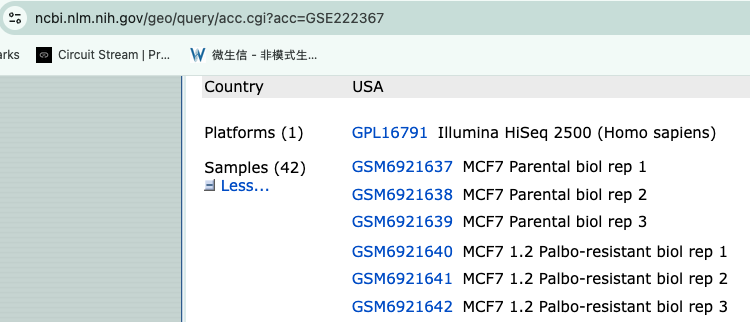
\includegraphics[width=0.6\linewidth]{image/GEOscreenshot} \caption{GEO dataset}\label{fig:fig-mychart}
\end{figure}

\chapter*{Differential Expression}\label{differential-expression}
\addcontentsline{toc}{chapter}{Differential Expression}

\textbf{This work is licensed under a \href{https://creativecommons.org/licenses/by-sa/4.0/deed.en}{Creative Commons Attribution-ShareAlike 4.0 Unported License}. This means that you are able to copy, share and modify the work, as long as the result is distributed under the same license.}

We perform differential expression analysis using a negative binomial generalized linear model using the edgeR package.

\section{Install and load libraries}\label{install-and-load-libraries}

\begin{Shaded}
\begin{Highlighting}[]
\DocumentationTok{\#\# CRAN and Bioconductor setup}
\ControlFlowTok{if}\NormalTok{ (}\SpecialCharTok{!}\FunctionTok{requireNamespace}\NormalTok{(}\StringTok{"BiocManager"}\NormalTok{, }\AttributeTok{quietly =} \ConstantTok{TRUE}\NormalTok{))}
  \FunctionTok{install.packages}\NormalTok{(}\StringTok{"BiocManager"}\NormalTok{)}

\DocumentationTok{\#\# List of CRAN packages}
\NormalTok{cran\_packages }\OtherTok{\textless{}{-}} \FunctionTok{c}\NormalTok{(}
  \StringTok{"tidyverse"}\NormalTok{,}
  \StringTok{"ggrepel"}
\NormalTok{)}

\CommentTok{\# List of Bioconductor packages}
\NormalTok{bioc\_packages }\OtherTok{\textless{}{-}} \FunctionTok{c}\NormalTok{(}
  \StringTok{"edgeR"}
\NormalTok{)}

\CommentTok{\# Install CRAN packages if not already installed}
\ControlFlowTok{for}\NormalTok{ (pkg }\ControlFlowTok{in}\NormalTok{ cran\_packages) \{}
  \ControlFlowTok{if}\NormalTok{ (}\SpecialCharTok{!}\FunctionTok{requireNamespace}\NormalTok{(pkg, }\AttributeTok{quietly =} \ConstantTok{TRUE}\NormalTok{)) \{}
    \FunctionTok{install.packages}\NormalTok{(pkg)}
\NormalTok{  \}}
\NormalTok{\}}

\CommentTok{\# Install Bioconductor packages if not already installed}
\ControlFlowTok{for}\NormalTok{ (pkg }\ControlFlowTok{in}\NormalTok{ bioc\_packages) \{}
  \ControlFlowTok{if}\NormalTok{ (}\SpecialCharTok{!}\FunctionTok{requireNamespace}\NormalTok{(pkg, }\AttributeTok{quietly =} \ConstantTok{TRUE}\NormalTok{)) \{}
\NormalTok{    BiocManager}\SpecialCharTok{::}\FunctionTok{install}\NormalTok{(pkg)}
\NormalTok{  \}}
\NormalTok{\}}

\CommentTok{\# Load the libraries}

\CommentTok{\# CRAN packages}
\FunctionTok{library}\NormalTok{(tidyverse)}
\end{Highlighting}
\end{Shaded}

\begin{verbatim}
## -- Attaching core tidyverse packages ------------------------ tidyverse 2.0.0 --
## v dplyr     1.2.1     v readr     2.2.0
## v forcats   1.0.1     v stringr   1.6.0
## v ggplot2   4.0.3     v tibble    3.3.1
## v lubridate 1.9.5     v tidyr     1.3.2
## v purrr     1.2.2     
## -- Conflicts ------------------------------------------ tidyverse_conflicts() --
## x dplyr::filter() masks stats::filter()
## x dplyr::lag()    masks stats::lag()
## i Use the conflicted package (<http://conflicted.r-lib.org/>) to force all conflicts to become errors
\end{verbatim}

\begin{Shaded}
\begin{Highlighting}[]
\FunctionTok{library}\NormalTok{(ggrepel)}
\CommentTok{\# Bioconductor packages}
\FunctionTok{library}\NormalTok{(edgeR)}
\end{Highlighting}
\end{Shaded}

\begin{verbatim}
## Loading required package: limma
\end{verbatim}

\begin{Shaded}
\begin{Highlighting}[]
\CommentTok{\# create the results folder (if it does not exist yet) to save the outputs}
\FunctionTok{dir.create}\NormalTok{(}\StringTok{"results"}\NormalTok{, }\AttributeTok{showWarnings =} \ConstantTok{FALSE}\NormalTok{)}
\end{Highlighting}
\end{Shaded}

\section{Data used for this comparison}\label{data-used-for-this-comparison}

For this analysis, we are going to compare the Palbo-resistant cell lines (3 biological replicates) versus the parental cell lines (3 biological replicates)

\begin{figure}
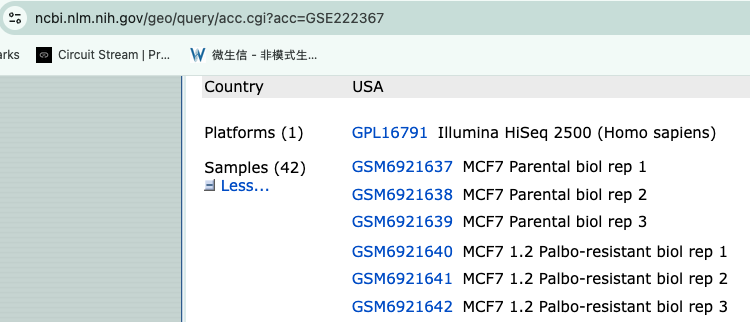
\includegraphics[width=0.6\linewidth]{image/GEOscreenshot} \caption{GEO dataset}\label{fig:dataset}
\end{figure}

\subsection{generate a DGE object}\label{generate-a-dge-object}

\begin{Shaded}
\begin{Highlighting}[]
\CommentTok{\# 1. Find the count files}
\NormalTok{files }\OtherTok{\textless{}{-}} \FunctionTok{list.files}\NormalTok{(}\AttributeTok{path =} \StringTok{"data"}\NormalTok{, }\AttributeTok{pattern =} \StringTok{"}\SpecialCharTok{\textbackslash{}\textbackslash{}}\StringTok{.txt}\SpecialCharTok{\textbackslash{}\textbackslash{}}\StringTok{.gz$"}\NormalTok{, }\AttributeTok{full.names =} \ConstantTok{TRUE}\NormalTok{)}

\CommentTok{\# 2. Sample names from the file names (strip the extension)}
\NormalTok{samples }\OtherTok{\textless{}{-}} \FunctionTok{sub}\NormalTok{(}\StringTok{"\_S.*"}\NormalTok{, }\StringTok{""}\NormalTok{, }\FunctionTok{basename}\NormalTok{(files))}

\CommentTok{\# 3. Read the files into a DGEList}
\CommentTok{\#    HTSeq output has no header: column 1 = gene ID, column 2 = count.}
\CommentTok{\#    R reads gzipped files directly, so no need to decompress.}
\NormalTok{dge }\OtherTok{\textless{}{-}} \FunctionTok{readDGE}\NormalTok{(files, }\AttributeTok{columns =} \FunctionTok{c}\NormalTok{(}\DecValTok{1}\NormalTok{, }\DecValTok{2}\NormalTok{), }\AttributeTok{header =} \ConstantTok{FALSE}\NormalTok{, }\AttributeTok{labels =}\NormalTok{ samples)}
\end{Highlighting}
\end{Shaded}

\begin{verbatim}
## Meta tags detected: __no_feature, __ambiguous, __too_low_aQual, __not_aligned, __alignment_not_unique
\end{verbatim}

\begin{Shaded}
\begin{Highlighting}[]
\CommentTok{\# 4. Remove HTSeq summary rows (\_\_no\_feature, \_\_ambiguous, etc.)}
\NormalTok{dge }\OtherTok{\textless{}{-}}\NormalTok{ dge[}\SpecialCharTok{!}\FunctionTok{grepl}\NormalTok{(}\StringTok{"\^{}\_\_"}\NormalTok{, }\FunctionTok{rownames}\NormalTok{(dge)), , keep.lib.sizes }\OtherTok{=} \ConstantTok{FALSE}\NormalTok{]}

\CommentTok{\# 5. (Optional) add group information}
\NormalTok{dge}\SpecialCharTok{$}\NormalTok{samples}\SpecialCharTok{$}\NormalTok{group }\OtherTok{\textless{}{-}} \FunctionTok{factor}\NormalTok{(}
  \FunctionTok{c}\NormalTok{(}\StringTok{"parental"}\NormalTok{, }\StringTok{"parental"}\NormalTok{, }\StringTok{"parental"}\NormalTok{,}
    \StringTok{"palbo\_resistant"}\NormalTok{, }\StringTok{"palbo\_resistant"}\NormalTok{, }\StringTok{"palbo\_resistant"}\NormalTok{),}
  \AttributeTok{levels =} \FunctionTok{c}\NormalTok{(}\StringTok{"parental"}\NormalTok{, }\StringTok{"palbo\_resistant"}\NormalTok{)   }\CommentTok{\# parental = reference}
\NormalTok{)}
\end{Highlighting}
\end{Shaded}

\section{Filter low-count genes and TMM-normalize}\label{filter-low-count-genes-and-tmm-normalize}

\begin{Shaded}
\begin{Highlighting}[]
\NormalTok{keep }\OtherTok{\textless{}{-}} \FunctionTok{filterByExpr}\NormalTok{(dge, }\AttributeTok{group =}\NormalTok{ dge}\SpecialCharTok{$}\NormalTok{samples}\SpecialCharTok{$}\NormalTok{group)}
\NormalTok{dge  }\OtherTok{\textless{}{-}}\NormalTok{ dge[keep, , keep.lib.sizes }\OtherTok{=} \ConstantTok{FALSE}\NormalTok{]}
\NormalTok{dge  }\OtherTok{\textless{}{-}} \FunctionTok{calcNormFactors}\NormalTok{(dge, }\AttributeTok{method =} \StringTok{"TMM"}\NormalTok{)}
\FunctionTok{cat}\NormalTok{(}\StringTok{"Genes retained after filtering:"}\NormalTok{, }\FunctionTok{nrow}\NormalTok{(dge), }\StringTok{"}\SpecialCharTok{\textbackslash{}n}\StringTok{"}\NormalTok{)}
\end{Highlighting}
\end{Shaded}

\begin{verbatim}
## Genes retained after filtering: 15246
\end{verbatim}

\begin{Shaded}
\begin{Highlighting}[]
\NormalTok{mds }\OtherTok{\textless{}{-}} \FunctionTok{plotMDS}\NormalTok{(dge, }\AttributeTok{col =} \FunctionTok{as.numeric}\NormalTok{(dge}\SpecialCharTok{$}\NormalTok{samples}\SpecialCharTok{$}\NormalTok{group), }\AttributeTok{main =} \StringTok{"MDS (logCPM)"}\NormalTok{)}
\end{Highlighting}
\end{Shaded}

\begin{Shaded}
\begin{Highlighting}[]
\NormalTok{group }\OtherTok{=}\NormalTok{ dge}\SpecialCharTok{$}\NormalTok{samples}\SpecialCharTok{$}\NormalTok{group}
\NormalTok{var\_pct }\OtherTok{\textless{}{-}} \FunctionTok{round}\NormalTok{(}\DecValTok{100} \SpecialCharTok{*}\NormalTok{ mds}\SpecialCharTok{$}\NormalTok{var.explained[mds}\SpecialCharTok{$}\NormalTok{dim.plot])}
\NormalTok{mds\_df }\OtherTok{\textless{}{-}} \FunctionTok{data.frame}\NormalTok{(}\AttributeTok{dim1 =}\NormalTok{ mds}\SpecialCharTok{$}\NormalTok{x, }\AttributeTok{dim2 =}\NormalTok{ mds}\SpecialCharTok{$}\NormalTok{y,}
                      \AttributeTok{sample =} \FunctionTok{colnames}\NormalTok{(dge), }\AttributeTok{group =}\NormalTok{ group)}

\FunctionTok{ggplot}\NormalTok{(mds\_df, }\FunctionTok{aes}\NormalTok{(}\AttributeTok{x =}\NormalTok{ dim1, }\AttributeTok{y =}\NormalTok{ dim2, }\AttributeTok{color =}\NormalTok{ group)) }\SpecialCharTok{+}
  \FunctionTok{geom\_point}\NormalTok{(}\AttributeTok{size =} \DecValTok{3}\NormalTok{) }\SpecialCharTok{+}
\NormalTok{  ggrepel}\SpecialCharTok{::}\FunctionTok{geom\_text\_repel}\NormalTok{(}\FunctionTok{aes}\NormalTok{(}\AttributeTok{label =}\NormalTok{ sample), }\AttributeTok{size =} \DecValTok{3}\NormalTok{, }\AttributeTok{color =} \StringTok{"grey30"}\NormalTok{,}
                            \AttributeTok{show.legend =} \ConstantTok{FALSE}\NormalTok{, }\AttributeTok{max.overlaps =} \ConstantTok{Inf}\NormalTok{,}
                            \AttributeTok{box.padding =} \FloatTok{0.4}\NormalTok{, }\AttributeTok{segment.color =} \StringTok{"grey60"}\NormalTok{) }\SpecialCharTok{+}
  \FunctionTok{labs}\NormalTok{(}\AttributeTok{title =} \StringTok{"MDS plot (all samples)"}\NormalTok{,}
       \AttributeTok{x =} \FunctionTok{sprintf}\NormalTok{(}\StringTok{"Leading logFC dim \%d (\%d\%\%)"}\NormalTok{, mds}\SpecialCharTok{$}\NormalTok{dim.plot[}\DecValTok{1}\NormalTok{], var\_pct[}\DecValTok{1}\NormalTok{]),}
       \AttributeTok{y =} \FunctionTok{sprintf}\NormalTok{(}\StringTok{"Leading logFC dim \%d (\%d\%\%)"}\NormalTok{, mds}\SpecialCharTok{$}\NormalTok{dim.plot[}\DecValTok{2}\NormalTok{], var\_pct[}\DecValTok{2}\NormalTok{]),}
       \AttributeTok{color =} \StringTok{"Group"}\NormalTok{) }\SpecialCharTok{+}
  \FunctionTok{theme\_minimal}\NormalTok{(}\AttributeTok{base\_size =} \DecValTok{12}\NormalTok{) }\SpecialCharTok{+}
  \FunctionTok{theme}\NormalTok{(}\AttributeTok{legend.position =} \StringTok{"right"}\NormalTok{)}
\end{Highlighting}
\end{Shaded}

\includegraphics{_main_files/figure-latex/unnamed-chunk-5-1.pdf}

\section{Design (\textasciitilde0 + group) and named contrast}\label{design-0-group-and-named-contrast}

\begin{Shaded}
\begin{Highlighting}[]
\NormalTok{design }\OtherTok{\textless{}{-}} \FunctionTok{model.matrix}\NormalTok{(}\SpecialCharTok{\textasciitilde{}} \DecValTok{0} \SpecialCharTok{+}\NormalTok{ group, }\AttributeTok{data =}\NormalTok{ dge}\SpecialCharTok{$}\NormalTok{samples)}
\FunctionTok{colnames}\NormalTok{(design) }\OtherTok{\textless{}{-}} \FunctionTok{levels}\NormalTok{(dge}\SpecialCharTok{$}\NormalTok{samples}\SpecialCharTok{$}\NormalTok{group)   }\CommentTok{\# "parental", "palbo\_resistant"}
 
\NormalTok{contr }\OtherTok{\textless{}{-}} \FunctionTok{makeContrasts}\NormalTok{(}
  \AttributeTok{resistant\_vs\_parental =}\NormalTok{ palbo\_resistant }\SpecialCharTok{{-}}\NormalTok{ parental,   }\CommentTok{\# + logFC = up in resistant}
  \AttributeTok{levels =}\NormalTok{ design}
\NormalTok{)}

\FunctionTok{head}\NormalTok{(design)}
\end{Highlighting}
\end{Shaded}

\begin{verbatim}
##            parental palbo_resistant
## GSM6921637        1               0
## GSM6921638        1               0
## GSM6921639        1               0
## GSM6921640        0               1
## GSM6921641        0               1
## GSM6921642        0               1
\end{verbatim}

\section{Dispersion estimation and quasi-likelihood GLM}\label{dispersion-estimation-and-quasi-likelihood-glm}

\begin{Shaded}
\begin{Highlighting}[]
\NormalTok{dge }\OtherTok{\textless{}{-}} \FunctionTok{estimateDisp}\NormalTok{(dge, design, }\AttributeTok{robust =} \ConstantTok{TRUE}\NormalTok{)}
\NormalTok{fit }\OtherTok{\textless{}{-}} \FunctionTok{glmQLFit}\NormalTok{(dge, design, }\AttributeTok{robust =} \ConstantTok{TRUE}\NormalTok{)}
 
\FunctionTok{par}\NormalTok{(}\AttributeTok{mfrow =} \FunctionTok{c}\NormalTok{(}\DecValTok{1}\NormalTok{, }\DecValTok{2}\NormalTok{)); }\FunctionTok{plotBCV}\NormalTok{(dge); }\FunctionTok{plotQLDisp}\NormalTok{(fit)}
\end{Highlighting}
\end{Shaded}

\includegraphics{_main_files/figure-latex/unnamed-chunk-7-1.pdf}

\begin{Shaded}
\begin{Highlighting}[]
\NormalTok{qlf }\OtherTok{\textless{}{-}} \FunctionTok{glmQLFTest}\NormalTok{(fit, }\AttributeTok{contrast =}\NormalTok{ contr[, }\StringTok{"resistant\_vs\_parental"}\NormalTok{])}
 
\NormalTok{res }\OtherTok{\textless{}{-}} \FunctionTok{topTags}\NormalTok{(qlf, }\AttributeTok{n =} \ConstantTok{Inf}\NormalTok{, }\AttributeTok{sort.by =} \StringTok{"PValue"}\NormalTok{)}\SpecialCharTok{$}\NormalTok{table}
\NormalTok{res}\SpecialCharTok{$}\NormalTok{gene }\OtherTok{\textless{}{-}} \FunctionTok{rownames}\NormalTok{(res)}
\end{Highlighting}
\end{Shaded}

\section{Calculating ranking score and export full results}\label{calculating-ranking-score-and-export-full-results}

\begin{Shaded}
\begin{Highlighting}[]
\NormalTok{res}\SpecialCharTok{$}\NormalTok{score }\OtherTok{=} \FunctionTok{sign}\NormalTok{(res}\SpecialCharTok{$}\NormalTok{logFC) }\SpecialCharTok{*} \SpecialCharTok{{-}}\FunctionTok{log10}\NormalTok{(res}\SpecialCharTok{$}\NormalTok{PValue)}
\FunctionTok{head}\NormalTok{(res)}
\end{Highlighting}
\end{Shaded}

\begin{verbatim}
##            logFC   logCPM        F       PValue          FDR  gene     score
## FOXA1  -7.733381 7.036614 212.9072 7.319997e-08 0.0003543738 FOXA1 -7.135489
## ESRP1 -12.579669 6.455576 208.4055 8.469988e-08 0.0003543738 ESRP1 -7.072117
## AZGP1 -11.099954 7.258554 184.8560 1.464633e-07 0.0003543738 AZGP1 -6.834271
## EPN3  -11.064332 6.286707 169.9951 2.143977e-07 0.0003543738  EPN3 -6.668780
## AP1M2 -12.059269 6.763487 169.5441 2.169978e-07 0.0003543738 AP1M2 -6.663545
## CAV1   10.118680 6.613522 165.7532 2.404307e-07 0.0003543738  CAV1  6.619010
\end{verbatim}

\#\#visualization

\begin{Shaded}
\begin{Highlighting}[]
\DocumentationTok{\#\#\# histogram of the ranking score}
\FunctionTok{hist}\NormalTok{(res}\SpecialCharTok{$}\NormalTok{score, }\AttributeTok{breaks=}\DecValTok{100}\NormalTok{, }\AttributeTok{col=}\StringTok{"orchid"}\NormalTok{, }\AttributeTok{xlab =} \StringTok{"score"}\NormalTok{, }\AttributeTok{main =} \StringTok{"Histogram of score"}\NormalTok{)}
\end{Highlighting}
\end{Shaded}

\includegraphics{_main_files/figure-latex/unnamed-chunk-9-1.pdf}

\begin{Shaded}
\begin{Highlighting}[]
\DocumentationTok{\#\#\# volcano plot}
\end{Highlighting}
\end{Shaded}

\begin{Shaded}
\begin{Highlighting}[]
\CommentTok{\# Step 1: add {-}log10(FDR), and label each gene Up / Down / Not sig}
\NormalTok{res }\OtherTok{\textless{}{-}}\NormalTok{ res }\SpecialCharTok{\%\textgreater{}\%}
  \FunctionTok{mutate}\NormalTok{(}
    \AttributeTok{negLogFDR =} \SpecialCharTok{{-}}\FunctionTok{log10}\NormalTok{(FDR),}
    \AttributeTok{status =} \FunctionTok{case\_when}\NormalTok{(}
\NormalTok{      FDR }\SpecialCharTok{\textless{}} \FloatTok{0.05} \SpecialCharTok{\&}\NormalTok{ logFC }\SpecialCharTok{\textgreater{}} \DecValTok{0} \SpecialCharTok{\textasciitilde{}} \StringTok{"Up"}\NormalTok{,}
\NormalTok{      FDR }\SpecialCharTok{\textless{}} \FloatTok{0.05} \SpecialCharTok{\&}\NormalTok{ logFC }\SpecialCharTok{\textless{}} \DecValTok{0} \SpecialCharTok{\textasciitilde{}} \StringTok{"Down"}\NormalTok{,}
      \ConstantTok{TRUE} \SpecialCharTok{\textasciitilde{}} \StringTok{"Not sig"}
\NormalTok{    )}
\NormalTok{  )}

\CommentTok{\# Step 2: pick the top 15 most significant genes on each side, to label}
\NormalTok{top\_up   }\OtherTok{\textless{}{-}}\NormalTok{ res }\SpecialCharTok{\%\textgreater{}\%} \FunctionTok{filter}\NormalTok{(status }\SpecialCharTok{==} \StringTok{"Up"}\NormalTok{)   }\SpecialCharTok{\%\textgreater{}\%} \FunctionTok{arrange}\NormalTok{(FDR) }\SpecialCharTok{\%\textgreater{}\%} \FunctionTok{slice\_head}\NormalTok{(}\AttributeTok{n =} \DecValTok{15}\NormalTok{)}
\NormalTok{top\_down }\OtherTok{\textless{}{-}}\NormalTok{ res }\SpecialCharTok{\%\textgreater{}\%} \FunctionTok{filter}\NormalTok{(status }\SpecialCharTok{==} \StringTok{"Down"}\NormalTok{) }\SpecialCharTok{\%\textgreater{}\%} \FunctionTok{arrange}\NormalTok{(FDR) }\SpecialCharTok{\%\textgreater{}\%} \FunctionTok{slice\_head}\NormalTok{(}\AttributeTok{n =} \DecValTok{15}\NormalTok{)}
\NormalTok{top\_genes }\OtherTok{\textless{}{-}} \FunctionTok{bind\_rows}\NormalTok{(top\_up, top\_down)}

\CommentTok{\# Step 3: plot}
\FunctionTok{ggplot}\NormalTok{(res, }\FunctionTok{aes}\NormalTok{(}\AttributeTok{x =}\NormalTok{ logFC, }\AttributeTok{y =}\NormalTok{ negLogFDR, }\AttributeTok{color =}\NormalTok{ status)) }\SpecialCharTok{+}
  \FunctionTok{geom\_point}\NormalTok{() }\SpecialCharTok{+}
  \FunctionTok{scale\_color\_manual}\NormalTok{(}\AttributeTok{values =} \FunctionTok{c}\NormalTok{(}\StringTok{"Up"} \OtherTok{=} \StringTok{"\#D55E00"}\NormalTok{, }\StringTok{"Down"} \OtherTok{=} \StringTok{"\#0072B2"}\NormalTok{, }\StringTok{"Not sig"} \OtherTok{=} \StringTok{"grey"}\NormalTok{)) }\SpecialCharTok{+}
\NormalTok{ ggrepel}\SpecialCharTok{::}\FunctionTok{geom\_text\_repel}\NormalTok{(}\AttributeTok{data =}\NormalTok{ top\_genes, }\FunctionTok{aes}\NormalTok{(}\AttributeTok{label =}\NormalTok{ gene), }\AttributeTok{max.overlaps =} \ConstantTok{Inf}\NormalTok{) }\SpecialCharTok{+}
  \FunctionTok{labs}\NormalTok{(}\AttributeTok{x =} \StringTok{"log2 Fold Change"}\NormalTok{, }\AttributeTok{y =} \StringTok{"{-}log10(FDR)"}\NormalTok{, }\AttributeTok{color =} \StringTok{"Status"}\NormalTok{)}\SpecialCharTok{+}
  \FunctionTok{coord\_cartesian}\NormalTok{(}\AttributeTok{ylim =} \FunctionTok{c}\NormalTok{(}\DecValTok{0}\NormalTok{, }\FloatTok{4.5}\NormalTok{)) }\SpecialCharTok{+}
  \FunctionTok{theme\_classic}\NormalTok{()}
\end{Highlighting}
\end{Shaded}

\includegraphics{_main_files/figure-latex/volcano-1.pdf}

\section{Result output}\label{result-output}

\begin{Shaded}
\begin{Highlighting}[]
\FunctionTok{print}\NormalTok{(}\FunctionTok{summary}\NormalTok{(}\FunctionTok{decideTests}\NormalTok{(qlf, }\AttributeTok{adjust.method =} \StringTok{"BH"}\NormalTok{, }\AttributeTok{p.value =} \FloatTok{0.05}\NormalTok{)))}
\end{Highlighting}
\end{Shaded}

\begin{verbatim}
##        -1*parental 1*palbo_resistant
## Down                            1325
## NotSig                         12579
## Up                              1342
\end{verbatim}

\begin{Shaded}
\begin{Highlighting}[]
\FunctionTok{write.csv}\NormalTok{(res, }\StringTok{"results/edgeR\_resistant\_vs\_parental\_all\_genes.csv"}\NormalTok{, }\AttributeTok{row.names =} \ConstantTok{FALSE}\NormalTok{)}
\end{Highlighting}
\end{Shaded}

\section{Version of packages and R}\label{version-of-packages-and-r}

\begin{Shaded}
\begin{Highlighting}[]
\FunctionTok{sessionInfo}\NormalTok{()}
\end{Highlighting}
\end{Shaded}

\begin{verbatim}
## R version 4.3.2 (2023-10-31)
## Platform: aarch64-apple-darwin20 (64-bit)
## Running under: macOS 15.5
## 
## Matrix products: default
## BLAS:   /Library/Frameworks/R.framework/Versions/4.3-arm64/Resources/lib/libRblas.0.dylib 
## LAPACK: /Library/Frameworks/R.framework/Versions/4.3-arm64/Resources/lib/libRlapack.dylib;  LAPACK version 3.11.0
## 
## locale:
## [1] en_US.UTF-8/en_US.UTF-8/en_US.UTF-8/C/en_US.UTF-8/en_US.UTF-8
## 
## time zone: America/Toronto
## tzcode source: internal
## 
## attached base packages:
## [1] stats     graphics  grDevices datasets  utils     methods   base     
## 
## other attached packages:
##  [1] edgeR_4.0.16    limma_3.58.1    ggrepel_0.9.8   lubridate_1.9.5
##  [5] forcats_1.0.1   stringr_1.6.0   dplyr_1.2.1     purrr_1.2.2    
##  [9] readr_2.2.0     tidyr_1.3.2     tibble_3.3.1    ggplot2_4.0.3  
## [13] tidyverse_2.0.0
## 
## loaded via a namespace (and not attached):
##  [1] generics_0.1.4      renv_1.2.4          stringi_1.8.9      
##  [4] lattice_0.22-7      hms_1.1.4           digest_0.6.39      
##  [7] magrittr_2.0.5      evaluate_1.0.5      grid_4.3.2         
## [10] timechange_0.4.0    RColorBrewer_1.1-3  bookdown_0.48      
## [13] fastmap_1.2.0       tinytex_0.61        BiocManager_1.30.27
## [16] scales_1.4.0        cli_3.6.6           rlang_1.3.0        
## [19] splines_4.3.2       withr_3.0.3         yaml_2.3.12        
## [22] otel_0.2.0          tools_4.3.2         tzdb_0.5.0         
## [25] locfit_1.5-9.12     vctrs_0.7.3         R6_2.6.1           
## [28] lifecycle_1.0.5     pkgconfig_2.0.3     pillar_1.11.1      
## [31] gtable_0.3.6        glue_1.8.1          Rcpp_1.1.2         
## [34] statmod_1.5.2       xfun_0.61           tidyselect_1.2.1   
## [37] rstudioapi_0.19.0   knitr_1.52          farver_2.1.2       
## [40] htmltools_0.5.9     labeling_0.4.3      rmarkdown_2.32     
## [43] compiler_4.3.2      S7_0.2.2
\end{verbatim}

\chapter*{Defined genelist}\label{defined-genelist}
\addcontentsline{toc}{chapter}{Defined genelist}

\textbf{This work is licensed under a \href{https://creativecommons.org/licenses/by-sa/4.0/deed.en}{Creative Commons Attribution-ShareAlike 4.0 Unported License}. This means that you are able to copy, share and modify the work, as long as the result is distributed under the same license.}

Authors: Veronique Voisin, Ruth Isserlin

Presenter: Veronique Voisin

\section{Introduction}\label{introduction}

During this practical lab, we will perform pathway enrichment analysis using a defined gene list.

\section{Goal of the exercise 1}\label{goal-of-the-exercise-1}

For this exercise, our goal is to run pathway enrichment analysis using g:Profiler and explore the results.
g:Profiler performs a gene-set enrichment analysis using a hypergeometric test (Fisher's exact test). The \href{http://geneontology.org/}{Gene Ontology} Biological Process, \href{https://reactome.org/}{Reactome} and \href{https://www.wikipathways.org/}{WikiPathways} sources are going to be used as pathway databases.
We wil also upload our custom geneset file.

g:Profiler can be used using the website at \url{https://biit.cs.ut.ee/gprofiler/gost}. However, for this practical lab, we will run it from the g:Profiler R package.

We will run the query and explore the table of results and visualize the results as bar and dot plots.

One of the greatest features of \href{https://biit.cs.ut.ee/gprofiler/gost}{g:Profiler} is that it is updated on a regular basis and most of the previous versions are available online ont the \href{https://biit.cs.ut.ee/gprofiler/page/archives}{gprofiler archive}.

The \href{https://biit.cs.ut.ee/gprofiler/page/r}{gprofielr2} -\href{https://biit.cs.ut.ee/gprofiler/gost}{g:Profiler} R implementation is a wrapper for the web version. You require an internet connection to get enrichment results.

\section{Data}\label{data}

g:Profiler requires a list of genes. For this analysis, we used genes we found to be differentially expressed in palbociclib-resistant samples compared with parental samples from the breast cancer cell line MCF7 (see chapter 1.

\section{Exercise 1 - prepare the gene lists}\label{exercise-1-defined}

This exercise requires the file ``edgeR\_resistant\_vs\_parental\_all\_genes.csv'' located in the results folder.

\subsection{Step 1 - Install and Load libraries}\label{step-1---install-and-load-libraries}

\begin{Shaded}
\begin{Highlighting}[]
\CommentTok{\# List of CRAN packages}
\NormalTok{cran\_packages }\OtherTok{\textless{}{-}} \FunctionTok{c}\NormalTok{(}
  \StringTok{"tidyverse"}\NormalTok{,}
  \StringTok{"knitr"}\NormalTok{,}
  \StringTok{"kableExtra"}\NormalTok{,}
  \StringTok{"glue"}\NormalTok{,}
  \StringTok{"patchwork"}\NormalTok{,}
  \StringTok{"ggdendro"}\NormalTok{,}
  \StringTok{"pheatmap"}\NormalTok{,}
  \StringTok{"gprofiler2"}\NormalTok{,}
  \StringTok{"GSA"}
\NormalTok{)}
\CommentTok{\# Install CRAN packages if not already installed}
\ControlFlowTok{for}\NormalTok{ (pkg }\ControlFlowTok{in}\NormalTok{ cran\_packages) \{}
  \ControlFlowTok{if}\NormalTok{ (}\SpecialCharTok{!}\FunctionTok{requireNamespace}\NormalTok{(pkg, }\AttributeTok{quietly =} \ConstantTok{TRUE}\NormalTok{)) \{}
    \FunctionTok{install.packages}\NormalTok{(pkg)}
\NormalTok{  \}}
\NormalTok{\}}
\CommentTok{\# Load the libraries}
\FunctionTok{library}\NormalTok{(tidyverse)}
\FunctionTok{library}\NormalTok{(knitr)}
\FunctionTok{library}\NormalTok{(kableExtra)}
\FunctionTok{library}\NormalTok{(glue)}
\FunctionTok{library}\NormalTok{(patchwork)}
\FunctionTok{library}\NormalTok{(ggdendro)}
\FunctionTok{library}\NormalTok{(pheatmap)}
\FunctionTok{library}\NormalTok{(gprofiler2)}
\FunctionTok{library}\NormalTok{(GSA)}

\CommentTok{\# create the results folder (if it does not exist yet) to save the outputs}
\FunctionTok{dir.create}\NormalTok{(}\StringTok{"results"}\NormalTok{, }\AttributeTok{showWarnings =} \ConstantTok{FALSE}\NormalTok{)}
\end{Highlighting}
\end{Shaded}

\subsection{Step 2 - Prepare the define gene lists}\label{step-2---prepare-the-define-gene-lists}

\begin{Shaded}
\begin{Highlighting}[]
\NormalTok{res }\OtherTok{=} \FunctionTok{read.csv}\NormalTok{(}\StringTok{"results/edgeR\_resistant\_vs\_parental\_all\_genes.csv"}\NormalTok{)}

\NormalTok{UPgenes }\OtherTok{\textless{}{-}}\NormalTok{ res}\SpecialCharTok{$}\NormalTok{gene[res}\SpecialCharTok{$}\NormalTok{logFC}\SpecialCharTok{\textgreater{}}\DecValTok{0} \SpecialCharTok{\&}\NormalTok{  res}\SpecialCharTok{$}\NormalTok{FDR }\SpecialCharTok{\textless{}=} \FloatTok{0.001}\NormalTok{]}
\NormalTok{DOWNgenes }\OtherTok{\textless{}{-}}\NormalTok{ res}\SpecialCharTok{$}\NormalTok{gene[res}\SpecialCharTok{$}\NormalTok{logFC}\SpecialCharTok{\textless{}}\DecValTok{0} \SpecialCharTok{\&}\NormalTok{  res}\SpecialCharTok{$}\NormalTok{FDR }\SpecialCharTok{\textless{}=} \FloatTok{0.001}\NormalTok{]}
\end{Highlighting}
\end{Shaded}

\subsection{Step 3 - Run g:Profiler}\label{step-3---run-gprofiler}

The next step is to run pathway enrichment analysis using \href{https://biit.cs.ut.ee/gprofiler/gost}{gost g:Profiler} using the g:Profiler2 R package.
For detailed descriptions of all the parameters that can be specified for the gost g:profiler function see the R package information - \href{https://cran.r-project.org/web/packages/gprofiler2/index.html}{here} and \href{https://rdrr.io/cran/gprofiler2/man/gost.html}{here}.

For this query we are specifying -

\begin{itemize}
\tightlist
\item
  query - the set of genes of interest, as loaded in from the gene list file (\texttt{query\_set}).
\item
  significant - set to FALSE because we want g:Profiler to return all the results not just the ones that it deems significant by its predetermined threshold. We will filter the results for significance in a next step.
\item
  ordered\_query - set to FALSE (because we are not taking into account the order of the list)
\item
  exclude\_iea - set to TRUE. We are removing the electronic inferred annotations from the GO database
\item
  correction\_method - set to fdr. by default g:Profiler uses g:Scs
\item
  organism - set to ``hsapiens'' for homo sapiens. Organism names are constructed by concatenating the first letter of the name and the family name (according to gprofiler2 documentation)
\item
  source - the geneset source databases to use for the analysis. We recommend using GO biological process (\url{GO:BP}), WikiPathways (WP) and Reactome (Reac) but there are additional sources you can add (GO molecular function or cellular component(\url{GO:MF}, \url{GO:CC}), KEGG, transcription factors (TF), microRNA targets (MIRNA), corum complexes (CORUM), Human protein atlas (HPA),Human phenotype ontology (HP) )
\end{itemize}

\subsubsection{run g:Profiler with the up genes}\label{run-gprofiler-with-the-up-genes}

\begin{Shaded}
\begin{Highlighting}[]
\NormalTok{query\_set }\OtherTok{=}\NormalTok{ UPgenes }

\NormalTok{gprofiler\_results\_UPgenes }\OtherTok{\textless{}{-}} \FunctionTok{gost}\NormalTok{(}\AttributeTok{query =}\NormalTok{ query\_set ,}
                          \AttributeTok{significant=}\ConstantTok{TRUE}\NormalTok{,}
                          \AttributeTok{ordered\_query =} \ConstantTok{FALSE}\NormalTok{,}
                          \AttributeTok{exclude\_iea=}\ConstantTok{TRUE}\NormalTok{,}
                          \AttributeTok{correction\_method =} \StringTok{"fdr"}\NormalTok{,}
                          \AttributeTok{organism =} \StringTok{"hsapiens"}\NormalTok{,}
                          \AttributeTok{source =} \FunctionTok{c}\NormalTok{(}\StringTok{"REAC"}\NormalTok{,}\StringTok{"WP"}\NormalTok{,}\StringTok{"GO:BP"}\NormalTok{))}
\end{Highlighting}
\end{Shaded}

\subsubsection{observe the results}\label{observe-the-results}

\begin{Shaded}
\begin{Highlighting}[]
\CommentTok{\#get the gprofiler results table}
\NormalTok{enrichment\_results }\OtherTok{\textless{}{-}}\NormalTok{ gprofiler\_results\_UPgenes}\SpecialCharTok{$}\NormalTok{result}

\CommentTok{\#display the names of all columns}
\FunctionTok{colnames}\NormalTok{(enrichment\_results)}
\end{Highlighting}
\end{Shaded}

\begin{verbatim}
##  [1] "query"                 "significant"           "p_value"              
##  [4] "term_size"             "query_size"            "intersection_size"    
##  [7] "precision"             "recall"                "term_id"              
## [10] "source"                "term_name"             "effective_domain_size"
## [13] "source_order"          "parents"
\end{verbatim}

\begin{Shaded}
\begin{Highlighting}[]
\CommentTok{\#display the top rows}
\FunctionTok{head}\NormalTok{(enrichment\_results)}
\end{Highlighting}
\end{Shaded}

\begin{verbatim}
##     query significant     p_value term_size query_size intersection_size
## 1 query_1        TRUE 0.005977645       635         74                13
## 2 query_1        TRUE 0.005977645       509         74                11
## 3 query_1        TRUE 0.005977645        61         74                 5
## 4 query_1        TRUE 0.005977645      1013         74                16
## 5 query_1        TRUE 0.005977645       188         74                 7
## 6 query_1        TRUE 0.005977645        73         74                 5
##    precision     recall    term_id source
## 1 0.17567568 0.02047244 GO:0035295  GO:BP
## 2 0.14864865 0.02161100 GO:0001944  GO:BP
## 3 0.06756757 0.08196721 GO:0050818  GO:BP
## 4 0.21621622 0.01579467 GO:2000026  GO:BP
## 5 0.09459459 0.03723404 GO:0050817  GO:BP
## 6 0.06756757 0.06849315 GO:0032963  GO:BP
##                                            term_name effective_domain_size
## 1                                   tube development                 16180
## 2                            vasculature development                 16180
## 3                          regulation of coagulation                 16180
## 4 regulation of multicellular organismal development                 16180
## 5                                        coagulation                 16180
## 6                         collagen metabolic process                 16180
##   source_order                            parents
## 1         8374             GO:0007275, GO:0048856
## 2          542             GO:0048731, GO:0072359
## 3        12418             GO:0050817, GO:0051239
## 4        23538 GO:0007275, GO:0050793, GO:0051239
## 5        12417                         GO:0032501
## 6         7434                         GO:0008152
\end{verbatim}

\subsubsection{YOUR TURN: run g:Profiler with the down genes (use same parameters as above)}\label{your-turn-run-gprofiler-with-the-down-genes-use-same-parameters-as-above}

\begin{Shaded}
\begin{Highlighting}[]
\DocumentationTok{\#\#Tip: remove eval=FALSE chunk option to run the code}
\NormalTok{query\_set }\OtherTok{=}\NormalTok{ XXXX}

\NormalTok{gprofiler\_results\_DOWNgenes }\OtherTok{\textless{}{-}} \FunctionTok{gost}\NormalTok{(}\AttributeTok{query =}\NormalTok{ XXXX,}
                          \AttributeTok{significant =}\NormalTok{ XXXX,}
                          \AttributeTok{ordered\_query =}\NormalTok{ XXXX,}
                          \AttributeTok{exclude\_iea =}\NormalTok{ XXXX,}
                          \AttributeTok{correction\_method =}\NormalTok{ XXXX,}
                          \AttributeTok{organism =}\NormalTok{ XXXX,}
                          \AttributeTok{source =} \FunctionTok{c}\NormalTok{(}\StringTok{"XXXX"}\NormalTok{,}\StringTok{"XXXX"}\NormalTok{,}\StringTok{"XXXX"}\NormalTok{))}

\DocumentationTok{\#\#observe the results (same as for the UP genes)}
\end{Highlighting}
\end{Shaded}

\subsection{Clear visualization of the results}\label{clear-visualization-of-the-results}

The enrichment\_results dataframe contains different columns. Let's rearrange the table to display the most important information. We will arrange the table so it contains: the database origin, the name of each of the pathway, term size , query size, intersection size and adjusted pvalue. -

\begin{itemize}
\tightlist
\item
  Term size: number of genes in the pathway as it is in the database
\item
  Query size: number of genes in our gene list
\item
  Intersection size: number of genes overlapping between our gene list and the tested pathway
\item
  pvalue: adjusted pvalue (corrected for multiple hypothesis testing using the Benjamini-Hochberg method)
\end{itemize}

The results are ordered by significance, from the most significant pathway (lowest p-value) to the least significant.

\begin{Shaded}
\begin{Highlighting}[]
\NormalTok{enrichment\_results }\OtherTok{\textless{}{-}}\NormalTok{ gprofiler\_results\_UPgenes}\SpecialCharTok{$}\NormalTok{result}
\NormalTok{enrichment\_results}\SpecialCharTok{$}\NormalTok{p\_value }\OtherTok{\textless{}{-}} \FunctionTok{formatC}\NormalTok{(enrichment\_results}\SpecialCharTok{$}\NormalTok{p\_value, }\AttributeTok{format =} \StringTok{"e"}\NormalTok{, }\AttributeTok{digits =} \DecValTok{2}\NormalTok{)}

\NormalTok{enrichment\_results }\OtherTok{=}\NormalTok{ enrichment\_results[ , }\FunctionTok{c}\NormalTok{(}\StringTok{"source"}\NormalTok{, }\StringTok{"term\_name"}\NormalTok{, }\StringTok{"term\_size"}\NormalTok{, }\StringTok{"query\_size"}\NormalTok{, }\StringTok{"intersection\_size"}\NormalTok{, }\StringTok{"p\_value"}\NormalTok{)]}

\FunctionTok{kable}\NormalTok{(}\FunctionTok{head}\NormalTok{(enrichment\_results, }\AttributeTok{n=}\DecValTok{20}\NormalTok{), }\AttributeTok{caption =} \StringTok{"Enrichment Result"}\NormalTok{) }\SpecialCharTok{\%\textgreater{}\%}
\FunctionTok{kable\_styling}\NormalTok{(}\AttributeTok{bootstrap\_options =} \FunctionTok{c}\NormalTok{(}\StringTok{"striped"}\NormalTok{, }\StringTok{"condensed"}\NormalTok{), }\AttributeTok{font\_size =} \DecValTok{10}\NormalTok{)}
\end{Highlighting}
\end{Shaded}

\begin{table}
\centering
\caption{\label{tab:unnamed-chunk-16}Enrichment Result}
\centering
\fontsize{10}{12}\selectfont
\begin{tabular}[t]{l|l|r|r|r|l}
\hline
source & term\_name & term\_size & query\_size & intersection\_size & p\_value\\
\hline
GO:BP & tube development & 635 & 74 & 13 & 5.98e-03\\
\hline
GO:BP & vasculature development & 509 & 74 & 11 & 5.98e-03\\
\hline
GO:BP & regulation of coagulation & 61 & 74 & 5 & 5.98e-03\\
\hline
GO:BP & regulation of multicellular organismal development & 1013 & 74 & 16 & 5.98e-03\\
\hline
GO:BP & coagulation & 188 & 74 & 7 & 5.98e-03\\
\hline
GO:BP & collagen metabolic process & 73 & 74 & 5 & 5.98e-03\\
\hline
GO:BP & anatomical structure morphogenesis & 1847 & 74 & 22 & 5.98e-03\\
\hline
GO:BP & cell adhesion mediated by integrin & 80 & 74 & 5 & 7.04e-03\\
\hline
GO:BP & blood vessel morphogenesis & 457 & 74 & 10 & 8.11e-03\\
\hline
GO:BP & tube morphogenesis & 562 & 74 & 11 & 8.11e-03\\
\hline
GO:BP & regulation of multicellular organismal process & 2293 & 74 & 24 & 8.15e-03\\
\hline
GO:BP & blood vessel development & 487 & 74 & 10 & 1.04e-02\\
\hline
GO:BP & positive regulation of blood coagulation & 21 & 74 & 3 & 1.44e-02\\
\hline
GO:BP & positive regulation of hemostasis & 21 & 74 & 3 & 1.44e-02\\
\hline
GO:BP & circulatory system development & 745 & 74 & 12 & 1.45e-02\\
\hline
GO:BP & regulation of blood coagulation & 57 & 74 & 4 & 1.45e-02\\
\hline
GO:BP & regulation of hemostasis & 58 & 74 & 4 & 1.46e-02\\
\hline
GO:BP & wound healing & 340 & 74 & 8 & 1.46e-02\\
\hline
GO:BP & positive regulation of coagulation & 23 & 74 & 3 & 1.46e-02\\
\hline
GO:BP & blood coagulation & 182 & 74 & 6 & 1.61e-02\\
\hline
\end{tabular}
\end{table}

\subsubsection{YOUR TURN: visualize the results with the down genes (use same parameters as above)}\label{your-turn-visualize-the-results-with-the-down-genes-use-same-parameters-as-above}

\begin{Shaded}
\begin{Highlighting}[]
\DocumentationTok{\#\#Tip: remove eval=FALSE chunk option to run the code}

\NormalTok{enrichment\_results }\OtherTok{\textless{}{-}}\NormalTok{ XXXX}
\NormalTok{enrichment\_results}\SpecialCharTok{$}\NormalTok{p\_value }\OtherTok{\textless{}{-}} \FunctionTok{formatC}\NormalTok{(XXXX)}

\NormalTok{enrichment\_results }\OtherTok{=}\NormalTok{ enrichment\_results[ , }\FunctionTok{c}\NormalTok{(}\StringTok{"XXXX"}\NormalTok{, }\StringTok{"XXXX"}\NormalTok{, }\StringTok{"XXXX"}\NormalTok{, }\StringTok{"XXXX"}\NormalTok{, }\StringTok{"XXXX"}\NormalTok{, }\StringTok{"XXXX"}\NormalTok{)]}

\FunctionTok{kable}\NormalTok{(}\FunctionTok{head}\NormalTok{(enrichment\_results, }\AttributeTok{n=}\DecValTok{20}\NormalTok{), }\AttributeTok{caption =} \StringTok{"Enrichment Result"}\NormalTok{) }\SpecialCharTok{\%\textgreater{}\%}
\FunctionTok{kable\_styling}\NormalTok{(}\AttributeTok{bootstrap\_options =} \FunctionTok{c}\NormalTok{(}\StringTok{"striped"}\NormalTok{, }\StringTok{"condensed"}\NormalTok{), }\AttributeTok{font\_size =} \DecValTok{10}\NormalTok{)}
\end{Highlighting}
\end{Shaded}

\subsection{Step 4 - Explore top table of results}\label{step-4---explore-top-table-of-results}

For this analysis, we chose to use 3 databases: \url{GO:BP}, Reactome and Wikipathways.
If we look at the top table only, we are only going to see the results of \url{GO:BP} but it is interesting to look at the top results for each of the 3 databunique(enrichment\_results\$source)

\begin{Shaded}
\begin{Highlighting}[]
\NormalTok{enrichment\_results }\OtherTok{\textless{}{-}}\NormalTok{ gprofiler\_results\_UPgenes}\SpecialCharTok{$}\NormalTok{result}
\DocumentationTok{\#\#Get the name of the databases}
\FunctionTok{unique}\NormalTok{(enrichment\_results}\SpecialCharTok{$}\NormalTok{source) }
\end{Highlighting}
\end{Shaded}

\begin{verbatim}
## [1] "GO:BP" "REAC"  "WP"
\end{verbatim}

\begin{Shaded}
\begin{Highlighting}[]
\DocumentationTok{\#\#Filter the dataframe to retrieve only the Reactome results}
\NormalTok{enrichment\_results\_Reac }\OtherTok{\textless{}{-}}\NormalTok{ enrichment\_results }\SpecialCharTok{\%\textgreater{}\%}
  \FunctionTok{filter}\NormalTok{(source }\SpecialCharTok{==} \StringTok{"REAC"}\NormalTok{)}

\DocumentationTok{\#\#Now display the top 20 pathways}
\FunctionTok{kable}\NormalTok{(}\FunctionTok{head}\NormalTok{(enrichment\_results\_Reac, }\AttributeTok{n=}\DecValTok{20}\NormalTok{), }\AttributeTok{caption =} \StringTok{"Enrichment Result"}\NormalTok{) }\SpecialCharTok{\%\textgreater{}\%}
\FunctionTok{kable\_styling}\NormalTok{(}\AttributeTok{bootstrap\_options =} \FunctionTok{c}\NormalTok{(}\StringTok{"striped"}\NormalTok{, }\StringTok{"condensed"}\NormalTok{), }\AttributeTok{font\_size =} \DecValTok{10}\NormalTok{)}
\end{Highlighting}
\end{Shaded}

\begin{table}
\centering
\caption{\label{tab:unnamed-chunk-18}Enrichment Result}
\centering
\fontsize{10}{12}\selectfont
\begin{tabular}[t]{l|l|r|r|r|r|r|r|l|l|l|r|r|l}
\hline
query & significant & p\_value & term\_size & query\_size & intersection\_size & precision & recall & term\_id & source & term\_name & effective\_domain\_size & source\_order & parents\\
\hline
query\_1 & TRUE & 0.0000077 & 298 & 57 & 12 & 0.2105263 & 0.0402685 & REAC:R-HSA-1474244 & REAC & Extracellular matrix organization & 11056 & 930 & REAC:0000000\\
\hline
query\_1 & TRUE & 0.0008208 & 89 & 57 & 6 & 0.1052632 & 0.0674157 & REAC:R-HSA-1474290 & REAC & Collagen formation & 11056 & 403 & REAC:R-HSA-1474244\\
\hline
query\_1 & TRUE & 0.0021054 & 67 & 57 & 5 & 0.0877193 & 0.0746269 & REAC:R-HSA-1650814 & REAC & Collagen biosynthesis and modifying enzymes & 11056 & 400 & REAC:R-HSA-1474290\\
\hline
query\_1 & TRUE & 0.0029160 & 76 & 57 & 5 & 0.0877193 & 0.0657895 & REAC:R-HSA-3000178 & REAC & ECM proteoglycans & 11056 & 851 & REAC:R-HSA-1474244\\
\hline
query\_1 & TRUE & 0.0033756 & 44 & 57 & 4 & 0.0701754 & 0.0909091 & REAC:R-HSA-1566948 & REAC & Elastic fibre formation & 11056 & 875 & REAC:R-HSA-1474244\\
\hline
query\_1 & TRUE & 0.0033756 & 84 & 57 & 5 & 0.0877193 & 0.0595238 & REAC:R-HSA-216083 & REAC & Integrin cell surface interactions & 11056 & 1267 & REAC:R-HSA-1474244\\
\hline
query\_1 & TRUE & 0.0097759 & 60 & 57 & 4 & 0.0701754 & 0.0666667 & REAC:R-HSA-2022090 & REAC & Assembly of collagen fibrils and other multimeric structures & 11056 & 186 & REAC:R-HSA-1474290\\
\hline
query\_1 & TRUE & 0.0256174 & 140 & 57 & 5 & 0.0877193 & 0.0357143 & REAC:R-HSA-1474228 & REAC & Degradation of the extracellular matrix & 11056 & 748 & REAC:R-HSA-1474244\\
\hline
query\_1 & TRUE & 0.0316913 & 39 & 57 & 3 & 0.0526316 & 0.0769231 & REAC:R-HSA-140877 & REAC & Formation of Fibrin Clot (Clotting Cascade) & 11056 & 986 & REAC:R-HSA-109582\\
\hline
query\_1 & TRUE & 0.0322168 & 42 & 57 & 3 & 0.0526316 & 0.0714286 & REAC:R-HSA-419037 & REAC & NCAM1 interactions & 11056 & 1577 & REAC:R-HSA-375165\\
\hline
query\_1 & TRUE & 0.0322168 & 516 & 57 & 9 & 0.1578947 & 0.0174419 & REAC:R-HSA-9006934 & REAC & Signaling by Receptor Tyrosine Kinases & 11056 & 2399 & REAC:R-HSA-162582\\
\hline
query\_1 & TRUE & 0.0338224 & 44 & 57 & 3 & 0.0526316 & 0.0681818 & REAC:R-HSA-8948216 & REAC & Collagen chain trimerization & 11056 & 401 & REAC:R-HSA-1650814\\
\hline
query\_1 & TRUE & 0.0449470 & 675 & 57 & 10 & 0.1754386 & 0.0148148 & REAC:R-HSA-109582 & REAC & Hemostasis & 11056 & 1168 & REAC:0000000\\
\hline
\end{tabular}
\end{table}

\subsubsection{YOUR TURN: DISPLAY THE TOP 20 PATHWAYS FOR THE WIKIPATHWAY DATABASE (``WP'') and the down genes}\label{your-turn-display-the-top-20-pathways-for-the-wikipathway-database-wp-and-the-down-genes}

\begin{Shaded}
\begin{Highlighting}[]
\NormalTok{enrichment\_results }\OtherTok{\textless{}{-}}\NormalTok{ gprofiler\_results\_DOWNgenes}\SpecialCharTok{$}\NormalTok{result}
\DocumentationTok{\#\#Get the name of the databases}
\FunctionTok{unique}\NormalTok{(enrichment\_results}\SpecialCharTok{$}\NormalTok{source) }

\DocumentationTok{\#\#Filter the dataframe to retrieve only the Reactome results}
\NormalTok{enrichment\_results\_WP }\OtherTok{\textless{}{-}}\NormalTok{ enrichment\_results }\SpecialCharTok{\%\textgreater{}\%}
  \FunctionTok{XXXX}\NormalTok{(source }\SpecialCharTok{==} \StringTok{"XXXX"}\NormalTok{)}

\DocumentationTok{\#\#Now display the top 20 pathways}
\FunctionTok{kable}\NormalTok{(}\FunctionTok{head}\NormalTok{(enrichment\_results\_WP, }\AttributeTok{n=}\DecValTok{20}\NormalTok{), }\AttributeTok{caption =} \StringTok{"Enrichment Result"}\NormalTok{) }\SpecialCharTok{\%\textgreater{}\%}
\FunctionTok{kable\_styling}\NormalTok{(}\AttributeTok{bootstrap\_options =} \FunctionTok{c}\NormalTok{(}\StringTok{"striped"}\NormalTok{, }\StringTok{"condensed"}\NormalTok{), }\AttributeTok{font\_size =} \DecValTok{10}\NormalTok{)}
\end{Highlighting}
\end{Shaded}

\subsection{Step 5 - Filter results by geneset size}\label{step-5---filter-results-by-geneset-size}

Restrict the results to just the ones that have at maximum gene-set size of 1000 and a minimum gene-set size of 10 and with an adjusted pvalue of 0.05.-

\begin{itemize}
\tightlist
\item
  maximum gene-set size of 1000: will remove very generic pathway terms that are less informative like ``regulation of gene expression''
\item
  minimum gene-set size of 10: will remove small pathways where the pvalue is significant athough the overlap size is very small
\item
  p\_thres: aim is to retrieve only pathways that are significant under this adjusted pvalue threshold of 0.01 (1\% false positive)
\end{itemize}

\begin{Shaded}
\begin{Highlighting}[]
\NormalTok{enrichment\_results }\OtherTok{\textless{}{-}}\NormalTok{ gprofiler\_results\_UPgenes}\SpecialCharTok{$}\NormalTok{result }

\NormalTok{min\_gs\_size }\OtherTok{=} \DecValTok{10}
\NormalTok{max\_gs\_size }\OtherTok{=} \DecValTok{1000}
\NormalTok{p\_thres }\OtherTok{=} \FloatTok{0.01}
\CommentTok{\# filter by params defined above}
\CommentTok{\# by default we have set the max and min gs size to 250 and 3, respectively.}


\DocumentationTok{\#\#the pvalue was stored as a character vector, we have to transform back into a numerical vector to be able to use it to filter values}
\NormalTok{enrichment\_results}\SpecialCharTok{$}\NormalTok{p\_value }\OtherTok{\textless{}{-}} \FunctionTok{as.numeric}\NormalTok{(enrichment\_results}\SpecialCharTok{$}\NormalTok{p\_value) }

\NormalTok{enrichment\_results\_mxgssize\_1000\_min\_10\_adjp\_0\_01 }\OtherTok{\textless{}{-}} 
                        \FunctionTok{subset}\NormalTok{(enrichment\_results,}
\NormalTok{                                   term\_size }\SpecialCharTok{\textgreater{}=}\NormalTok{ min\_gs\_size }\SpecialCharTok{\&} 
\NormalTok{                                   term\_size }\SpecialCharTok{\textless{}=}\NormalTok{ max\_gs\_size }\SpecialCharTok{\&} 
\NormalTok{                                   p\_value }\SpecialCharTok{\textless{}=}\NormalTok{ p\_thres )}

\CommentTok{\#}
\NormalTok{myrows }\OtherTok{=} \FunctionTok{nrow}\NormalTok{(enrichment\_results\_mxgssize\_1000\_min\_10\_adjp\_0\_01)}

\FunctionTok{print}\NormalTok{(}\FunctionTok{glue}\NormalTok{(}\StringTok{"It results in \{myrows\} selected pathways with maximum gene{-}set size of \{max\_gs\_size\} and minimum gene{-}set of \{min\_gs\_size\} with an adjusted p{-}value of \{p\_thres\} . "}\NormalTok{))}
\end{Highlighting}
\end{Shaded}

\begin{verbatim}
## It results in 15 selected pathways with maximum gene-set size of 1000 and minimum gene-set of 10 with an adjusted p-value of 0.01 .
\end{verbatim}

\subsubsection{YOUR TURN: using the enrichment results for the down genes, use gene-set size filters and FDR filters and display the results}\label{your-turn-using-the-enrichment-results-for-the-down-genes-use-gene-set-size-filters-and-fdr-filters-and-display-the-results}

In a second step, try different thresholds of maximum gene-set size and adjusted pvalue threshold: 500 and 250 for * max\_gs\_size and 0.05 or 0.001 for pvalue-

\begin{itemize}
\tightlist
\item
  Option 1

  \begin{itemize}
  \tightlist
  \item
    max\_gs\_size = 500
  \item
    p\_thres = 0.001
  \end{itemize}
\end{itemize}

or

\begin{itemize}
\tightlist
\item
  Option 2

  \begin{itemize}
  \tightlist
  \item
    max\_gs\_size = 250
  \item
    p\_thres = 0.05
  \end{itemize}
\end{itemize}

How many pathways do you get for each option (nrow())??

\begin{Shaded}
\begin{Highlighting}[]
\NormalTok{enrichment\_results }\OtherTok{\textless{}{-}}\NormalTok{ gprofiler\_results\_DOWNgenes}\SpecialCharTok{$}\NormalTok{result }

\NormalTok{min\_gs\_size }\OtherTok{=}\NormalTok{ XXXX}
\NormalTok{max\_gs\_size }\OtherTok{=}\NormalTok{ XXXX}
\NormalTok{p\_thres }\OtherTok{=}\NormalTok{ XXXX}
\CommentTok{\# filter by params defined above}
\CommentTok{\# by default we have set the max and min gs size to 250 and 3, respectively.}


\DocumentationTok{\#\#the pvalue was stored as a character vector, we have to transform back into a numerical vector to be able to use it to filter values}
\NormalTok{enrichment\_results}\SpecialCharTok{$}\NormalTok{p\_value }\OtherTok{\textless{}{-}} \FunctionTok{as.numeric}\NormalTok{(enrichment\_results}\SpecialCharTok{$}\NormalTok{p\_value) }

\NormalTok{enrichment\_results }\OtherTok{\textless{}{-}}\NormalTok{ XXXXX}
                        
\CommentTok{\#}
\NormalTok{myrows }\OtherTok{=} \FunctionTok{nrow}\NormalTok{(enrichment\_results)}

\FunctionTok{print}\NormalTok{(}\FunctionTok{glue}\NormalTok{(}\StringTok{"It results in \{myrows\} selected pathways with maximum gene{-}set size of \{max\_gs\_size\} and minimum gene{-}set of \{min\_gs\_size\} with an adjusted p{-}value of \{p\_thres\} . "}\NormalTok{))}
\end{Highlighting}
\end{Shaded}

\subsection{Step 6 - Run g:profiler with your own genesets (example using BaderLab genesets)}\label{step-6---run-gprofiler-with-your-own-genesets-example-using-baderlab-genesets}

With regards to pathway sets there are two options when using \href{https://biit.cs.ut.ee/gprofiler/gost}{g:Profiler} -

\begin{itemize}
\tightlist
\item
  Use the genesets that are supplied by \href{https://biit.cs.ut.ee/gprofiler/gost}{g:Profiler} as we just did.
\item
  Upload your own genesets.
\end{itemize}

The most common reasons for supplying your own genesets is the ability to use up to date annotations or in-house annotations that might not be available in the public sphere yet. It can be used to test the enrichment in a particular pathway of interest that might not be in the general pathway database but that you obtained for example by extracting the data from a published paper.
You need to format this pathway in a \href{https://www.gsea-msigdb.org/gsea/doc/GSEAUserGuideFrame.html}{.gmt file}.

In this example, we will upload the Baderlab gene set file that contains multiple database sources. We filtered the gene-set prior to uploading the gene-set file to g:Profiler.
The Baderlab gene set file combines different sources of databases and you can find more information at: \url{https://baderlab.org/GeneSets}

'\,`'Why do we filter the geneset before running gprofiler'\,'\,'

The g:Profiler interface only allows for filtering genesets by size only after the analysis is complete. After the analysis is complete means the filtering is happening after Multiple hypothesis testing. Filtering prior to the analysis will generate more robust results because we exclude the uninformative large genesets prior to testing changing the sets that multiple hypothesis filtering will get rid of.

We have 1 example of gmt files with different filtering thresholds :
* genesets less of equal than 500 genes

Load in the GMT file

This step will take the gmt file that wedownloaded locally and upload them into our R environment in the GSA.genesets object called ``genesets\_baderlab\_genesets''.
The capture.output() function is only there to redirect the printed messages for a clearer notebook.

The format of the GMT file is described \href{here}{https://software.broadinstitute.org/cancer/software/gsea/wiki/index.php/Data\_formats\#GMT:\emph{Gene\_Matrix\_Transposed\_file\_format}.28.2A.gmt.29} and consists of rows with the following

\begin{itemize}
\tightlist
\item
  Name
\item
  Description
\item
  tab delimited list of genes a part of this geneset
\end{itemize}

Write out the gmt file with genenames

In order to use your own genesets with g:Profiler you need to upload the the file to g:Profiler server first. The function will return an ID that you need to specify in the organism parameter of the g:Profiler gost function call.
It is done by using the upload\_GMT\_file() function which is included in the gprofiler2 package.
Note: it took about 2 minutes to run this chunck of code.

\begin{Shaded}
\begin{Highlighting}[]
\NormalTok{dest\_gmt\_file\_500 }\OtherTok{=}\StringTok{"data/Human\_GOBP\_AllPathways\_filtered\_500orLessV2.gmt"}

\NormalTok{custom\_gmt\_max500 }\OtherTok{\textless{}{-}} \FunctionTok{upload\_GMT\_file}\NormalTok{(}
                        \AttributeTok{gmtfile=}\NormalTok{dest\_gmt\_file\_500)}
\end{Highlighting}
\end{Shaded}

\begin{verbatim}
## Your custom annotations ID is gp__twiy_ALwk_UL0.
## You can use this ID as an 'organism' name in all the related enrichment tests against this custom source.
\end{verbatim}

\begin{verbatim}
## Just use: gost(my_genes, organism = 'gp__twiy_ALwk_UL0')
\end{verbatim}

\begin{Shaded}
\begin{Highlighting}[]
\NormalTok{UPgenes }\OtherTok{\textless{}{-}}\NormalTok{ res}\SpecialCharTok{$}\NormalTok{gene[res}\SpecialCharTok{$}\NormalTok{logFC}\SpecialCharTok{\textgreater{}}\DecValTok{0} \SpecialCharTok{\&}\NormalTok{  res}\SpecialCharTok{$}\NormalTok{FDR }\SpecialCharTok{\textless{}=} \FloatTok{0.001}\NormalTok{]}
\NormalTok{DOWNgenes }\OtherTok{\textless{}{-}}\NormalTok{ res}\SpecialCharTok{$}\NormalTok{gene[res}\SpecialCharTok{$}\NormalTok{logFC}\SpecialCharTok{\textless{}}\DecValTok{0} \SpecialCharTok{\&}\NormalTok{  res}\SpecialCharTok{$}\NormalTok{FDR }\SpecialCharTok{\textless{}=} \FloatTok{0.001}\NormalTok{]}


\NormalTok{gprofiler\_results\_custom\_max500\_UPgenes }\OtherTok{\textless{}{-}} \FunctionTok{gost}\NormalTok{(}\AttributeTok{query =}\NormalTok{ UPgenes  ,}
                                     \AttributeTok{significant=}\ConstantTok{TRUE}\NormalTok{,}
                                      \AttributeTok{ordered\_query =} \ConstantTok{FALSE}\NormalTok{,}
                                      \AttributeTok{exclude\_iea=}\ConstantTok{TRUE}\NormalTok{,}
                                     \AttributeTok{correction\_method =} \StringTok{"fdr"}\NormalTok{,}
                                 \AttributeTok{organism =}\NormalTok{ custom\_gmt\_max500}
\NormalTok{                                     )}
\end{Highlighting}
\end{Shaded}

\begin{verbatim}
## Detected custom GMT source request
\end{verbatim}

\begin{Shaded}
\begin{Highlighting}[]
\NormalTok{enrichment\_results\_UPgenes }\OtherTok{\textless{}{-}}\NormalTok{ gprofiler\_results\_custom\_max500\_UPgenes}\SpecialCharTok{$}\NormalTok{result}

\NormalTok{enrichment\_results\_UPgenes}\SpecialCharTok{$}\NormalTok{parents }\OtherTok{\textless{}{-}} \FunctionTok{sapply}\NormalTok{(}
\NormalTok{  enrichment\_results\_UPgenes}\SpecialCharTok{$}\NormalTok{parents,}
  \ControlFlowTok{function}\NormalTok{(x) }\FunctionTok{paste}\NormalTok{(x, }\AttributeTok{collapse =} \StringTok{", "}\NormalTok{)}
\NormalTok{)}
 
\DocumentationTok{\#\#Now display the top 20 pathways}
\FunctionTok{kable}\NormalTok{(}\FunctionTok{head}\NormalTok{(enrichment\_results\_UPgenes, }\AttributeTok{n=}\DecValTok{20}\NormalTok{), }\AttributeTok{caption =} \StringTok{"Enrichment Result"}\NormalTok{) }\SpecialCharTok{\%\textgreater{}\%}
\FunctionTok{kable\_styling}\NormalTok{(}\AttributeTok{bootstrap\_options =} \FunctionTok{c}\NormalTok{(}\StringTok{"striped"}\NormalTok{, }\StringTok{"condensed"}\NormalTok{), }\AttributeTok{font\_size =} \DecValTok{10}\NormalTok{)}
\end{Highlighting}
\end{Shaded}

\begin{table}
\centering
\caption{\label{tab:unnamed-chunk-22}Enrichment Result}
\centering
\fontsize{10}{12}\selectfont
\begin{tabular}[t]{l|l|r|r|r|r|r|r|l|l|l|r|r|l}
\hline
query & significant & p\_value & term\_size & query\_size & intersection\_size & precision & recall & term\_id & source & term\_name & effective\_domain\_size & source\_order & parents\\
\hline
query\_1 & TRUE & 0.0000025 & 308 & 81 & 13 & 0.1604938 & 0.0422078 & EXTRACELLULAR MATRIX ORGANIZATION\%REACTOME\%R-HSA-1474244.5 & Human\_GOBP\_AllPathways\_filtered\_500orLessV2 & Extracellular matrix organization & 17710 & 3114 & \\
\hline
query\_1 & TRUE & 0.0005125 & 66 & 81 & 6 & 0.0740741 & 0.0909091 & BETA1 INTEGRIN CELL SURFACE INTERACTIONS\%PATHWAY INTERACTION DATABASE NCI-NATURE CURATED DATA\%BETA1 INTEGRIN CELL SURFACE INTERACTIONS & Human\_GOBP\_AllPathways\_filtered\_500orLessV2 & Beta1 integrin cell surface interactions & 17710 & 1083 & \\
\hline
query\_1 & TRUE & 0.0020101 & 89 & 81 & 6 & 0.0740741 & 0.0674157 & COLLAGEN FORMATION\%REACTOME DATABASE ID RELEASE 97\%1474290 & Human\_GOBP\_AllPathways\_filtered\_500orLessV2 & Collagen formation & 17710 & 2582 & \\
\hline
query\_1 & TRUE & 0.0043121 & 62 & 81 & 5 & 0.0617284 & 0.0806452 & REGULATION OF COAGULATION\%GOBP\%GO:0050818 & Human\_GOBP\_AllPathways\_filtered\_500orLessV2 & regulation of coagulation & 17710 & 14756 & \\
\hline
query\_1 & TRUE & 0.0050573 & 67 & 81 & 5 & 0.0617284 & 0.0746269 & COLLAGEN BIOSYNTHESIS AND MODIFYING ENZYMES\%REACTOME DATABASE ID RELEASE 97\%1650814 & Human\_GOBP\_AllPathways\_filtered\_500orLessV2 & Collagen biosynthesis and modifying enzymes & 17710 & 3202 & \\
\hline
query\_1 & TRUE & 0.0067961 & 422 & 81 & 10 & 0.1234568 & 0.0236967 & TUBE DEVELOPMENT\%GOBP\%GO:0035295 & Human\_GOBP\_AllPathways\_filtered\_500orLessV2 & tube development & 17710 & 9957 & \\
\hline
query\_1 & TRUE & 0.0086573 & 40 & 81 & 4 & 0.0493827 & 0.1000000 & ELASTIC FIBRE FORMATION\%REACTOME DATABASE ID RELEASE 97\%1566948 & Human\_GOBP\_AllPathways\_filtered\_500orLessV2 & Elastic fibre formation & 17710 & 4843 & \\
\hline
query\_1 & TRUE & 0.0104444 & 283 & 81 & 8 & 0.0987654 & 0.0282686 & VASCULATURE DEVELOPMENT\%GOBP\%GO:0001944 & Human\_GOBP\_AllPathways\_filtered\_500orLessV2 & vasculature development & 17710 & 8945 & \\
\hline
query\_1 & TRUE & 0.0137184 & 57 & 81 & 4 & 0.0493827 & 0.0701754 & COAGULATION PATHWAY\%REACTOME DATABASE ID RELEASE 97\%9769740 & Human\_GOBP\_AllPathways\_filtered\_500orLessV2 & Coagulation pathway & 17710 & 2450 & \\
\hline
query\_1 & TRUE & 0.0137184 & 98 & 81 & 5 & 0.0617284 & 0.0510204 & POSITIVE REGULATION OF MONOATOMIC ION TRANSMEMBRANE TRANSPORT\%GOBP\%GO:0034767 & Human\_GOBP\_AllPathways\_filtered\_500orLessV2 & positive regulation of monoatomic ion transmembrane transport & 17710 & 7284 & \\
\hline
query\_1 & TRUE & 0.0137184 & 50 & 81 & 4 & 0.0493827 & 0.0800000 & REGULATION OF CLOTTING CASCADE\%REACTOME DATABASE ID RELEASE 97\%9769739 & Human\_GOBP\_AllPathways\_filtered\_500orLessV2 & Regulation of clotting cascade & 17710 & 4167 & \\
\hline
query\_1 & TRUE & 0.0137184 & 57 & 81 & 4 & 0.0493827 & 0.0701754 & REGULATION OF BLOOD COAGULATION\%GOBP\%GO:0030193 & Human\_GOBP\_AllPathways\_filtered\_500orLessV2 & regulation of blood coagulation & 17710 & 17655 & \\
\hline
query\_1 & TRUE & 0.0137184 & 21 & 81 & 3 & 0.0370370 & 0.1428571 & POSITIVE REGULATION OF HEMOSTASIS\%GOBP\%GO:1900048 & Human\_GOBP\_AllPathways\_filtered\_500orLessV2 & positive regulation of hemostasis & 17710 & 15624 & \\
\hline
query\_1 & TRUE & 0.0137184 & 240 & 81 & 7 & 0.0864198 & 0.0291667 & BLOOD VESSEL MORPHOGENESIS\%GOBP\%GO:0048514 & Human\_GOBP\_AllPathways\_filtered\_500orLessV2 & blood vessel morphogenesis & 17710 & 12918 & \\
\hline
query\_1 & TRUE & 0.0137184 & 94 & 81 & 5 & 0.0617284 & 0.0531915 & POSITIVE REGULATION OF CATION TRANSMEMBRANE TRANSPORT\%GOBP\%GO:1904064 & Human\_GOBP\_AllPathways\_filtered\_500orLessV2 & positive regulation of cation transmembrane transport & 17710 & 11849 & \\
\hline
query\_1 & TRUE & 0.0137184 & 56 & 81 & 4 & 0.0493827 & 0.0714286 & ASSEMBLY OF COLLAGEN FIBRILS AND OTHER MULTIMERIC STRUCTURES\%REACTOME DATABASE ID RELEASE 97\%2022090 & Human\_GOBP\_AllPathways\_filtered\_500orLessV2 & Assembly of collagen fibrils and other multimeric structures & 17710 & 4570 & \\
\hline
query\_1 & TRUE & 0.0137184 & 21 & 81 & 3 & 0.0370370 & 0.1428571 & POSITIVE REGULATION OF BLOOD COAGULATION\%GOBP\%GO:0030194 & Human\_GOBP\_AllPathways\_filtered\_500orLessV2 & positive regulation of blood coagulation & 17710 & 18367 & \\
\hline
query\_1 & TRUE & 0.0137184 & 52 & 81 & 4 & 0.0493827 & 0.0769231 & COLLAGEN METABOLIC PROCESS\%GOBP\%GO:0032963 & Human\_GOBP\_AllPathways\_filtered\_500orLessV2 & collagen metabolic process & 17710 & 16593 & \\
\hline
query\_1 & TRUE & 0.0139108 & 58 & 81 & 4 & 0.0493827 & 0.0689655 & REGULATION OF HEMOSTASIS\%GOBP\%GO:1900046 & Human\_GOBP\_AllPathways\_filtered\_500orLessV2 & regulation of hemostasis & 17710 & 7751 & \\
\hline
query\_1 & TRUE & 0.0141423 & 23 & 81 & 3 & 0.0370370 & 0.1304348 & POSITIVE REGULATION OF COAGULATION\%GOBP\%GO:0050820 & Human\_GOBP\_AllPathways\_filtered\_500orLessV2 & positive regulation of coagulation & 17710 & 12228 & \\
\hline
\end{tabular}
\end{table}

\begin{Shaded}
\begin{Highlighting}[]
\FunctionTok{write.csv}\NormalTok{( enrichment\_results\_UPgenes, }\StringTok{"results/enrichment\_results\_gprofiler\_UPgenes.csv"}\NormalTok{)}
\end{Highlighting}
\end{Shaded}

\subsubsection{YOUR TURN: perform the same task with the down genes}\label{your-turn-perform-the-same-task-with-the-down-genes}

\begin{Shaded}
\begin{Highlighting}[]
\NormalTok{gprofiler\_results\_custom\_max500\_DNgenes }\OtherTok{\textless{}{-}} \FunctionTok{gost}\NormalTok{(}
                                      \AttributeTok{query =}\NormalTok{ XXXX  ,}
                                     \AttributeTok{significant=}\NormalTok{XXXX,}
                                      \AttributeTok{ordered\_query =}\NormalTok{ XXXX,}
                                      \AttributeTok{exclude\_iea=}\NormalTok{XXXX,}
                                     \AttributeTok{correction\_method =} \StringTok{"XXX"}\NormalTok{,}
                                 \AttributeTok{organism =}\NormalTok{ XXXX}
\NormalTok{                                     )}

\NormalTok{enrichment\_results\_DNgenes }\OtherTok{\textless{}{-}}\NormalTok{ gprofiler\_results\_custom\_max500\_DNgenes}\SpecialCharTok{$}\NormalTok{result}


\NormalTok{enrichment\_results\_DNgenes}\SpecialCharTok{$}\NormalTok{parents }\OtherTok{\textless{}{-}} \FunctionTok{sapply}\NormalTok{(}
\NormalTok{  enrichment\_results\_DNgenes}\SpecialCharTok{$}\NormalTok{parents,}
  \ControlFlowTok{function}\NormalTok{(x) }\FunctionTok{paste}\NormalTok{(x, }\AttributeTok{collapse =} \StringTok{", "}\NormalTok{)}
\NormalTok{)}

\FunctionTok{kable}\NormalTok{(}\FunctionTok{head}\NormalTok{(enrichment\_results\_DNgenes, }\AttributeTok{n=}\DecValTok{20}\NormalTok{), }\AttributeTok{caption =} \StringTok{"Enrichment Result"}\NormalTok{) }\SpecialCharTok{\%\textgreater{}\%}
\FunctionTok{kable\_styling}\NormalTok{(}\AttributeTok{bootstrap\_options =} \FunctionTok{c}\NormalTok{(}\StringTok{"striped"}\NormalTok{, }\StringTok{"condensed"}\NormalTok{), }\AttributeTok{font\_size =} \DecValTok{10}\NormalTok{)}

\FunctionTok{write.csv}\NormalTok{( enrichment\_results\_DNgenes, }\StringTok{"results/enrichment\_results\_gprofiler\_DNgenes.csv"}\NormalTok{)}
\end{Highlighting}
\end{Shaded}

\section{Exercise 2 - visualization}\label{exercise-2---visualization}

We will use clusterProfiler style visualization.
\#\#\# Step 1 - Bar plot

\begin{Shaded}
\begin{Highlighting}[]
\DocumentationTok{\#\#Calculate a score (small very significant adjusted p value will turn into a large score)}

\NormalTok{enrichment\_results\_UPgenes }\OtherTok{\textless{}{-}}\NormalTok{ gprofiler\_results\_custom\_max500\_UPgenes}\SpecialCharTok{$}\NormalTok{result}

\NormalTok{enrichment\_results\_UPgenes}\SpecialCharTok{$}\NormalTok{score }\OtherTok{=} \SpecialCharTok{{-}}\FunctionTok{log10}\NormalTok{(}\FunctionTok{as.numeric}\NormalTok{(enrichment\_results\_UPgenes}\SpecialCharTok{$}\NormalTok{p\_value))}

\NormalTok{enrichment }\OtherTok{\textless{}{-}}\NormalTok{ enrichment\_results\_UPgenes }\SpecialCharTok{\%\textgreater{}\%}
  \FunctionTok{as\_tibble}\NormalTok{() }\SpecialCharTok{\%\textgreater{}\%}
  \FunctionTok{arrange}\NormalTok{(}\FunctionTok{desc}\NormalTok{(score)) }\SpecialCharTok{\%\textgreater{}\%}
  \FunctionTok{slice\_head}\NormalTok{(}\AttributeTok{n =} \DecValTok{20}\NormalTok{)}

\NormalTok{p }\OtherTok{=} \FunctionTok{ggplot}\NormalTok{(enrichment, }\FunctionTok{aes}\NormalTok{(}\FunctionTok{reorder}\NormalTok{(term\_name, score), score)) }\SpecialCharTok{+}
  \FunctionTok{geom\_col}\NormalTok{(}\FunctionTok{aes}\NormalTok{(}\AttributeTok{fill =}\NormalTok{ score), }\AttributeTok{width=}\FloatTok{0.8}\NormalTok{) }\SpecialCharTok{+}
  \FunctionTok{scale\_fill\_gradient}\NormalTok{(}\AttributeTok{low =} \StringTok{"\#C1F6F8"}\NormalTok{, }\AttributeTok{high =} \StringTok{"\#00BFC4"}\NormalTok{)}\SpecialCharTok{+}
  \FunctionTok{coord\_flip}\NormalTok{() }\SpecialCharTok{+}
  \FunctionTok{labs}\NormalTok{(}\AttributeTok{x=}\StringTok{""}\NormalTok{, }\AttributeTok{y=}\StringTok{"Normalized Enrichment Score"}\NormalTok{,}\AttributeTok{title=}\StringTok{"Pathway enrichment analysis "}\NormalTok{) }\SpecialCharTok{+} 
  \FunctionTok{theme\_minimal}\NormalTok{()}

\NormalTok{p}
\end{Highlighting}
\end{Shaded}

\includegraphics{_main_files/figure-latex/unnamed-chunk-24-1.pdf}

\subsection{Step 2 - Dot plot with segment}\label{step-2---dot-plot-with-segment}

\begin{Shaded}
\begin{Highlighting}[]
\NormalTok{enrichmentTop20 }\OtherTok{\textless{}{-}}\NormalTok{ enrichment }\SpecialCharTok{\%\textgreater{}\%}
  \FunctionTok{arrange}\NormalTok{(}\FunctionTok{desc}\NormalTok{(score)) }\SpecialCharTok{\%\textgreater{}\%}
  \FunctionTok{slice\_head}\NormalTok{(}\AttributeTok{n =} \DecValTok{20}\NormalTok{)}

\NormalTok{p }\OtherTok{=} \FunctionTok{ggplot}\NormalTok{(enrichmentTop20, }\FunctionTok{aes}\NormalTok{(}
  \AttributeTok{y =} \FunctionTok{fct\_reorder}\NormalTok{(term\_name, score),}
  \AttributeTok{x =}\NormalTok{ score,}
  \AttributeTok{color =}\NormalTok{ score,}
  \AttributeTok{size =}\NormalTok{ score}
\NormalTok{)) }\SpecialCharTok{+}
  \FunctionTok{geom\_point}\NormalTok{() }\SpecialCharTok{+}
  \FunctionTok{scale\_color\_gradientn}\NormalTok{(}
    \AttributeTok{colours =} \FunctionTok{c}\NormalTok{(}\StringTok{"\#56A443"}\NormalTok{, }\StringTok{"\#8AA443"}\NormalTok{, }\StringTok{"\#f7ca64"}\NormalTok{),}
    \AttributeTok{trans =} \StringTok{"log10"}\NormalTok{,}
    \AttributeTok{guide =} \FunctionTok{guide\_colorbar}\NormalTok{(}\AttributeTok{reverse =} \ConstantTok{FALSE}\NormalTok{, }\AttributeTok{order =} \DecValTok{1}\NormalTok{)}
\NormalTok{  ) }\SpecialCharTok{+}
  \FunctionTok{scale\_size\_continuous}\NormalTok{(}\AttributeTok{range =} \FunctionTok{c}\NormalTok{(}\DecValTok{4}\NormalTok{, }\DecValTok{8}\NormalTok{)) }\SpecialCharTok{+}
  \FunctionTok{theme\_bw}\NormalTok{(}\AttributeTok{base\_size =} \DecValTok{12}\NormalTok{) }\SpecialCharTok{+}
  \FunctionTok{xlab}\NormalTok{(}\StringTok{"score {-}log10(adj pvalue)"}\NormalTok{) }\SpecialCharTok{+}
  \FunctionTok{ylab}\NormalTok{(}\ConstantTok{NULL}\NormalTok{) }\SpecialCharTok{+}
  \FunctionTok{ggtitle}\NormalTok{(}\StringTok{"Pathway Enrichment Analysis"}\NormalTok{) }\SpecialCharTok{+}
  \FunctionTok{theme}\NormalTok{(}
    \AttributeTok{axis.text.y =} \FunctionTok{element\_text}\NormalTok{(}\AttributeTok{size =} \DecValTok{10}\NormalTok{)}
\NormalTok{  )}
\NormalTok{p}
\end{Highlighting}
\end{Shaded}

\includegraphics{_main_files/figure-latex/unnamed-chunk-25-1.pdf}

\subsection{Step 4 - Hierarchical Cluster}\label{step-4---hierarchical-cluster}

The problem with the earlier visualization, which represents the top 20 pathways, is that it does not account for the overlap between gene sets. As you can observe, many pathways have similar names because they share a substantial number of genes. To provide a more accurate and efficient representation of the results, and to obtain a quicker and clearer overview, it would be more appropriate to aggregate and summarize pathways with substantial gene overlap, thereby reducing redundancy.

Our first approach is to use hierarchical clustering based on a distance matrix that measures the similarity between pathways according to the number of genes they have in common, allowing us to visualize their relationships.

\begin{Shaded}
\begin{Highlighting}[]
\NormalTok{enrichment\_results\_UPgenes }\OtherTok{\textless{}{-}}\NormalTok{ gprofiler\_results\_custom\_max500\_UPgenes}\SpecialCharTok{$}\NormalTok{result}

\NormalTok{enrichment\_results\_UPgenes}\SpecialCharTok{$}\NormalTok{score }\OtherTok{=} \SpecialCharTok{{-}}\FunctionTok{log10}\NormalTok{(}\FunctionTok{as.numeric}\NormalTok{(enrichment\_results\_UPgenes}\SpecialCharTok{$}\NormalTok{p\_value))}

\CommentTok{\# Top 20 enriched terms}
\NormalTok{enrichmentTop20 }\OtherTok{\textless{}{-}}\NormalTok{ enrichment\_results\_UPgenes }\SpecialCharTok{\%\textgreater{}\%}
  \FunctionTok{arrange}\NormalTok{(}\FunctionTok{desc}\NormalTok{(score)) }\SpecialCharTok{\%\textgreater{}\%}
  \FunctionTok{slice\_head}\NormalTok{(}\AttributeTok{n =} \DecValTok{20}\NormalTok{)}
\end{Highlighting}
\end{Shaded}

\subsubsection{Get gene list in each pathway}\label{get-gene-list-in-each-pathway}

The genes contained in each pathway that overlap with our gene list are unfortunately not included in the enrichment results output. We therefore need to retrieve these genes from the pathway file by extracting the pathways of interest and merging them with our gene list.

addgenes: helper function to add gene list to enrichment result table

\begin{Shaded}
\begin{Highlighting}[]
\NormalTok{addgenes }\OtherTok{=} \ControlFlowTok{function}\NormalTok{(gmtfile, enrichmentresult )\{}


\NormalTok{capt\_output }\OtherTok{\textless{}{-}} \FunctionTok{capture.output}\NormalTok{(genesets\_baderlab\_genesets }\OtherTok{\textless{}{-}} 
                                \FunctionTok{GSA.read.gmt}\NormalTok{(}\AttributeTok{filename =}\NormalTok{ dest\_gmt\_file\_500))}

\FunctionTok{names}\NormalTok{(genesets\_baderlab\_genesets}\SpecialCharTok{$}\NormalTok{genesets) }\OtherTok{\textless{}{-}} 
\NormalTok{                                genesets\_baderlab\_genesets}\SpecialCharTok{$}\NormalTok{geneset.names}


\NormalTok{subset\_genesets }\OtherTok{\textless{}{-}}\NormalTok{ genesets\_baderlab\_genesets}\SpecialCharTok{$}\NormalTok{genesets[}\FunctionTok{which}\NormalTok{(genesets\_baderlab\_genesets}\SpecialCharTok{$}\NormalTok{geneset.names }\SpecialCharTok{\%in\%}\NormalTok{ enrichmentresult}\SpecialCharTok{$}\NormalTok{term\_id)]}

\NormalTok{genes }\OtherTok{\textless{}{-}} \FunctionTok{lapply}\NormalTok{(subset\_genesets,}\AttributeTok{FUN=}\ControlFlowTok{function}\NormalTok{(x)\{}\FunctionTok{intersect}\NormalTok{(x,query\_set)\})}

\CommentTok{\# For each of the genes collapse to the comma separate text}
\NormalTok{genes\_collapsed }\OtherTok{\textless{}{-}} \FunctionTok{unlist}\NormalTok{(}\FunctionTok{lapply}\NormalTok{(genes,}\AttributeTok{FUN=}\ControlFlowTok{function}\NormalTok{(x)\{}\FunctionTok{paste}\NormalTok{(x,}\AttributeTok{collapse =} \StringTok{","}\NormalTok{)\}))}
  
\NormalTok{genes\_collapsed\_df }\OtherTok{\textless{}{-}} \FunctionTok{data.frame}\NormalTok{(}
                            \AttributeTok{term\_id =} \FunctionTok{names}\NormalTok{(genes), }
                            \AttributeTok{genes =}\NormalTok{ genes\_collapsed,}\AttributeTok{stringsAsFactors =} \ConstantTok{FALSE}\NormalTok{)}
  


\NormalTok{formatted\_results }\OtherTok{\textless{}{-}} \FunctionTok{merge}\NormalTok{(enrichmentresult,genes\_collapsed\_df,}\AttributeTok{by.x=}\StringTok{"term\_id"}\NormalTok{ , }\AttributeTok{by.y=}\StringTok{"term\_id"}\NormalTok{ )}

\NormalTok{formatted\_results }\OtherTok{\textless{}{-}}\NormalTok{ formatted\_results[}\FunctionTok{order}\NormalTok{(formatted\_results}\SpecialCharTok{$}\NormalTok{p\_value),]}

\FunctionTok{return}\NormalTok{(formatted\_results)}
\NormalTok{\}}
\end{Highlighting}
\end{Shaded}

\subsubsection{Running the function to add genes}\label{running-the-function-to-add-genes}

\begin{Shaded}
\begin{Highlighting}[]
\NormalTok{formatted\_results }\OtherTok{\textless{}{-}} \FunctionTok{addgenes}\NormalTok{(}\AttributeTok{gmtfile =}\NormalTok{ dest\_gmt\_file\_500 , }\AttributeTok{enrichmentresult=}\NormalTok{ enrichment\_results\_UPgenes)}

\FunctionTok{head}\NormalTok{(formatted\_results)}
\end{Highlighting}
\end{Shaded}

\begin{verbatim}
##                                                                                                                                   term_id
## 18                                                                             EXTRACELLULAR MATRIX ORGANIZATION%REACTOME%R-HSA-1474244.5
## 2  BETA1 INTEGRIN CELL SURFACE INTERACTIONS%PATHWAY INTERACTION DATABASE NCI-NATURE CURATED DATA%BETA1 INTEGRIN CELL SURFACE INTERACTIONS
## 12                                                                             COLLAGEN FORMATION%REACTOME DATABASE ID RELEASE 97%1474290
## 42                                                                                              REGULATION OF COAGULATION%GOBP%GO:0050818
## 9                                                     COLLAGEN BIOSYNTHESIS AND MODIFYING ENZYMES%REACTOME DATABASE ID RELEASE 97%1650814
## 55                                                                                                       TUBE DEVELOPMENT%GOBP%GO:0035295
##      query significant      p_value term_size query_size intersection_size
## 18 query_1        TRUE 2.491195e-06       308         81                13
## 2  query_1        TRUE 5.124925e-04        66         81                 6
## 12 query_1        TRUE 2.010127e-03        89         81                 6
## 42 query_1        TRUE 4.312081e-03        62         81                 5
## 9  query_1        TRUE 5.057330e-03        67         81                 5
## 55 query_1        TRUE 6.796124e-03       422         81                10
##     precision     recall                                      source
## 18 0.16049383 0.04220779 Human_GOBP_AllPathways_filtered_500orLessV2
## 2  0.07407407 0.09090909 Human_GOBP_AllPathways_filtered_500orLessV2
## 12 0.07407407 0.06741573 Human_GOBP_AllPathways_filtered_500orLessV2
## 42 0.06172840 0.08064516 Human_GOBP_AllPathways_filtered_500orLessV2
## 9  0.06172840 0.07462687 Human_GOBP_AllPathways_filtered_500orLessV2
## 55 0.12345679 0.02369668 Human_GOBP_AllPathways_filtered_500orLessV2
##                                      term_name effective_domain_size
## 18           Extracellular matrix organization                 17710
## 2     Beta1 integrin cell surface interactions                 17710
## 12                          Collagen formation                 17710
## 42                   regulation of coagulation                 17710
## 9  Collagen biosynthesis and modifying enzymes                 17710
## 55                            tube development                 17710
##    source_order parents    score
## 18         3114    NULL 5.603592
## 2          1083    NULL 3.290313
## 12         2582    NULL 2.696776
## 42        14756    NULL 2.365313
## 9          3202    NULL 2.296079
## 55         9957    NULL 2.167739
##                                                                           genes
## 18 FBLN1,FBN1,SNTB1,ITGA5,TIMP2,P3H2,P3H3,LOX,COL6A2,COL6A1,COL5A1,SERPINE1,BGN
## 2                                         COL6A1,FBN1,ITGA5,TGFBI,COL5A1,COL6A2
## 12                                           P3H2,P3H3,LOX,COL6A2,COL6A1,COL5A1
## 42                                                   F2R,CAV1,PROCR,SERPINE1,F3
## 9                                                P3H2,P3H3,COL6A2,COL6A1,COL5A1
## 55                   ERRFI1,TGFBI,LOX,CLMP,SERPINE1,WNK4,ITGA5,RAMP1,CCBE1,CAV1
\end{verbatim}

\subsubsection{Calculating the distance matrix using the jaccard coefficient}\label{calculating-the-distance-matrix-using-the-jaccard-coefficient}

\begin{itemize}
\tightlist
\item
  Many pathways share genes, so similar biological processes can appear under different pathway names. To group similar pathways, we look at how many genes they have in common.
\item
  The Jaccard coefficient measures the shared genes relative to all unique genes in the two pathways, from 0 (no overlap) to 1 (identical).
\item
  The overlap coefficient measures the shared genes relative to the smaller pathway and shows when one pathway is mostly contained within another, from 0 (no overlap) to 1 (smaller pathway contained into larger one).
\end{itemize}

\begin{figure}
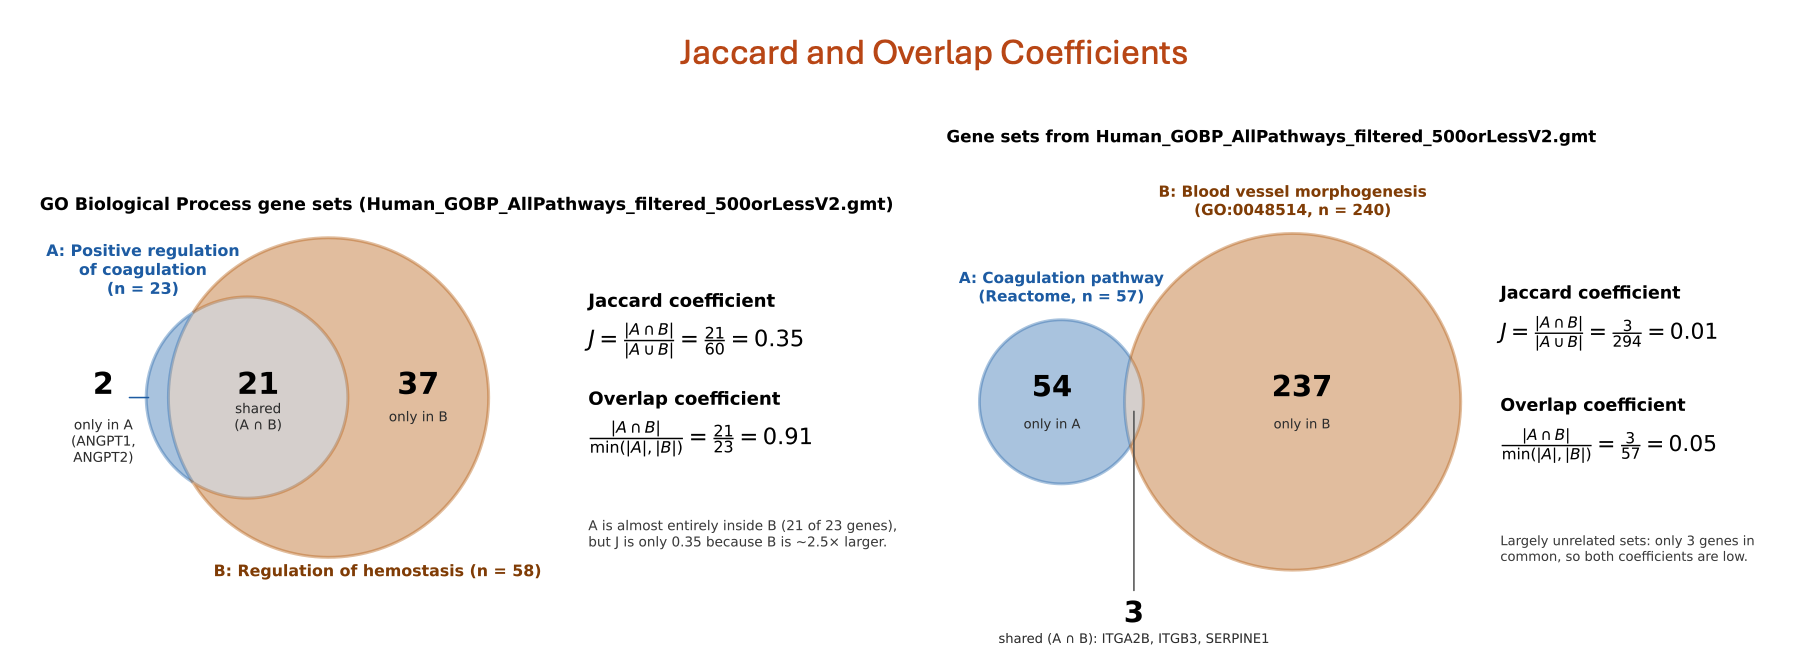
\includegraphics[width=1.1\linewidth]{image/jaccard_Overlap_coefficient} \caption{Jaccard and overlap coefficients for two gene sets.}\label{fig:jaccard-overlap}
\end{figure}

We convert these scores into distances (1 − score) and use them to group similar pathways into broader biological themes.

\#\#Illustration with Jaccard Coefficient

\begin{Shaded}
\begin{Highlighting}[]
\CommentTok{\# Convert genes to lists}
\NormalTok{gene\_lists }\OtherTok{\textless{}{-}} \FunctionTok{strsplit}\NormalTok{(formatted\_results}\SpecialCharTok{$}\NormalTok{genes, }\StringTok{","}\NormalTok{)}

\CommentTok{\# Calculate Jaccard similarity matrix}
\NormalTok{n }\OtherTok{\textless{}{-}} \FunctionTok{length}\NormalTok{(gene\_lists)}
\NormalTok{jaccard\_mat }\OtherTok{\textless{}{-}} \FunctionTok{matrix}\NormalTok{(}\DecValTok{0}\NormalTok{, n, n)}
\FunctionTok{rownames}\NormalTok{(jaccard\_mat) }\OtherTok{\textless{}{-}}\NormalTok{ formatted\_results}\SpecialCharTok{$}\NormalTok{term\_name}
\FunctionTok{colnames}\NormalTok{(jaccard\_mat) }\OtherTok{\textless{}{-}}\NormalTok{ formatted\_results}\SpecialCharTok{$}\NormalTok{term\_name}

\ControlFlowTok{for}\NormalTok{ (i }\ControlFlowTok{in} \FunctionTok{seq\_len}\NormalTok{(n)) \{}
  \ControlFlowTok{for}\NormalTok{ (j }\ControlFlowTok{in} \FunctionTok{seq\_len}\NormalTok{(n)) \{}
\NormalTok{    intersection }\OtherTok{\textless{}{-}} \FunctionTok{length}\NormalTok{(}\FunctionTok{intersect}\NormalTok{(gene\_lists[[i]], gene\_lists[[j]]))}
\NormalTok{    union        }\OtherTok{\textless{}{-}} \FunctionTok{length}\NormalTok{(}\FunctionTok{union}\NormalTok{(gene\_lists[[i]],     gene\_lists[[j]]))}
\NormalTok{    jaccard\_mat[i, j] }\OtherTok{\textless{}{-}}\NormalTok{ intersection }\SpecialCharTok{/}\NormalTok{ union}
\NormalTok{  \}}
\NormalTok{\}}


\NormalTok{labs }\OtherTok{\textless{}{-}}\NormalTok{ formatted\_results}\SpecialCharTok{$}\NormalTok{term\_name}
\NormalTok{labs }\OtherTok{\textless{}{-}} \FunctionTok{ifelse}\NormalTok{(}\FunctionTok{nchar}\NormalTok{(labs) }\SpecialCharTok{\textgreater{}} \DecValTok{30}\NormalTok{, }\FunctionTok{paste0}\NormalTok{(}\FunctionTok{substr}\NormalTok{(labs, }\DecValTok{1}\NormalTok{, }\DecValTok{27}\NormalTok{), }\StringTok{"..."}\NormalTok{), labs)}
\FunctionTok{rownames}\NormalTok{(jaccard\_mat) }\OtherTok{\textless{}{-}} \FunctionTok{colnames}\NormalTok{(jaccard\_mat) }\OtherTok{\textless{}{-}} \FunctionTok{make.unique}\NormalTok{(labs)}

\NormalTok{keep }\OtherTok{\textless{}{-}} \FunctionTok{sample}\NormalTok{(}\FunctionTok{seq\_len}\NormalTok{(}\FunctionTok{nrow}\NormalTok{(jaccard\_mat)), }\FunctionTok{min}\NormalTok{(}\DecValTok{20}\NormalTok{, }\FunctionTok{nrow}\NormalTok{(jaccard\_mat)))}
\NormalTok{jaccard\_sub }\OtherTok{\textless{}{-}}\NormalTok{ jaccard\_mat[keep, keep]}


\CommentTok{\# Heatmap}
\NormalTok{p }\OtherTok{\textless{}{-}} \FunctionTok{pheatmap}\NormalTok{(}
\NormalTok{  jaccard\_sub,}
  \AttributeTok{color           =} \FunctionTok{colorRampPalette}\NormalTok{(}\FunctionTok{c}\NormalTok{(}\StringTok{"white"}\NormalTok{, }\StringTok{"\#C6DBEF"}\NormalTok{, }\StringTok{"\#6BAED6"}\NormalTok{, }\StringTok{"\#2171B5"}\NormalTok{, }\StringTok{"\#08306B"}\NormalTok{))(}\DecValTok{100}\NormalTok{),}
  \AttributeTok{breaks          =} \FunctionTok{seq}\NormalTok{(}\DecValTok{0}\NormalTok{, }\DecValTok{1}\NormalTok{, }\AttributeTok{length.out =} \DecValTok{101}\NormalTok{),}
  \AttributeTok{display\_numbers =}\NormalTok{ F,}
  \CommentTok{\#number\_format   = "\%.2f",}
  \CommentTok{\#number\_color    = "black",}
  \CommentTok{\#fontsize\_number = 8,}
  \AttributeTok{clustering\_distance\_rows =} \FunctionTok{as.dist}\NormalTok{(}\DecValTok{1} \SpecialCharTok{{-}}\NormalTok{ jaccard\_sub),}
  \AttributeTok{clustering\_distance\_cols =} \FunctionTok{as.dist}\NormalTok{(}\DecValTok{1} \SpecialCharTok{{-}}\NormalTok{ jaccard\_sub),}
  \AttributeTok{border\_color    =} \StringTok{"grey90"}\NormalTok{,}
  \AttributeTok{fontsize\_row    =} \DecValTok{7}\NormalTok{,}
  \AttributeTok{fontsize\_col    =} \DecValTok{7}\NormalTok{,}
  \AttributeTok{angle\_col       =} \DecValTok{45}\NormalTok{,}
  \AttributeTok{main            =} \StringTok{"Jaccard coefficient (20 random gene sets)"}
\NormalTok{)}
\end{Highlighting}
\end{Shaded}

\includegraphics{_main_files/figure-latex/unnamed-chunk-29-1.pdf}

\#\#Illustration with Overlap Coefficient

\begin{Shaded}
\begin{Highlighting}[]
\CommentTok{\# Calculate Overlap coefficient matrix (reuses gene\_lists and n from above)}
\NormalTok{overlap\_mat }\OtherTok{\textless{}{-}} \FunctionTok{matrix}\NormalTok{(}\DecValTok{0}\NormalTok{, n, n)}

\ControlFlowTok{for}\NormalTok{ (i }\ControlFlowTok{in} \FunctionTok{seq\_len}\NormalTok{(n)) \{}
  \ControlFlowTok{for}\NormalTok{ (j }\ControlFlowTok{in} \FunctionTok{seq\_len}\NormalTok{(n)) \{}
\NormalTok{    intersection }\OtherTok{\textless{}{-}} \FunctionTok{length}\NormalTok{(}\FunctionTok{intersect}\NormalTok{(gene\_lists[[i]], gene\_lists[[j]]))}
\NormalTok{    smaller      }\OtherTok{\textless{}{-}} \FunctionTok{min}\NormalTok{(}\FunctionTok{length}\NormalTok{(gene\_lists[[i]]), }\FunctionTok{length}\NormalTok{(gene\_lists[[j]]))}
\NormalTok{    overlap\_mat[i, j] }\OtherTok{\textless{}{-}}\NormalTok{ intersection }\SpecialCharTok{/}\NormalTok{ smaller}
\NormalTok{  \}}
\NormalTok{\}}

\FunctionTok{rownames}\NormalTok{(overlap\_mat) }\OtherTok{\textless{}{-}} \FunctionTok{colnames}\NormalTok{(overlap\_mat) }\OtherTok{\textless{}{-}} \FunctionTok{make.unique}\NormalTok{(labs)}

\CommentTok{\# Use the same 20 gene sets as the Jaccard heatmap so the two can be compared}
\NormalTok{overlap\_sub }\OtherTok{\textless{}{-}}\NormalTok{ overlap\_mat[keep, keep]}


\CommentTok{\# Heatmap}
\NormalTok{p }\OtherTok{\textless{}{-}} \FunctionTok{pheatmap}\NormalTok{(}
\NormalTok{  overlap\_sub,}
  \AttributeTok{color           =} \FunctionTok{colorRampPalette}\NormalTok{(}\FunctionTok{c}\NormalTok{(}\StringTok{"white"}\NormalTok{, }\StringTok{"\#C6DBEF"}\NormalTok{, }\StringTok{"\#6BAED6"}\NormalTok{, }\StringTok{"\#2171B5"}\NormalTok{, }\StringTok{"\#08306B"}\NormalTok{))(}\DecValTok{100}\NormalTok{),}
  \AttributeTok{breaks          =} \FunctionTok{seq}\NormalTok{(}\DecValTok{0}\NormalTok{, }\DecValTok{1}\NormalTok{, }\AttributeTok{length.out =} \DecValTok{101}\NormalTok{),}
  \AttributeTok{display\_numbers =}\NormalTok{ F,}
  \AttributeTok{clustering\_distance\_rows =} \FunctionTok{as.dist}\NormalTok{(}\DecValTok{1} \SpecialCharTok{{-}}\NormalTok{ overlap\_sub),}
  \AttributeTok{clustering\_distance\_cols =} \FunctionTok{as.dist}\NormalTok{(}\DecValTok{1} \SpecialCharTok{{-}}\NormalTok{ overlap\_sub),}
  \AttributeTok{border\_color    =} \StringTok{"grey90"}\NormalTok{,}
  \AttributeTok{fontsize\_row    =} \DecValTok{7}\NormalTok{,}
  \AttributeTok{fontsize\_col    =} \DecValTok{7}\NormalTok{,}
  \AttributeTok{angle\_col       =} \DecValTok{45}\NormalTok{,}
  \AttributeTok{main            =} \StringTok{"Overlap coefficient (20 random gene sets)"}
\NormalTok{)}
\end{Highlighting}
\end{Shaded}

\includegraphics{_main_files/figure-latex/unnamed-chunk-30-1.pdf}

\#\#Hierarchical Clustering

plot\_hclust\_enrichment: helper function to cluster the top enriched pathways by gene overlap (Jaccard distance) and plot them next to the dendrogram

\begin{Shaded}
\begin{Highlighting}[]
\NormalTok{plot\_hclust\_enrichment }\OtherTok{=} \ControlFlowTok{function}\NormalTok{(enrichment\_results, }\AttributeTok{n\_top =} \DecValTok{20}\NormalTok{, }\AttributeTok{n\_clusters =} \DecValTok{8}\NormalTok{) \{}

\NormalTok{  enrichment\_results}\SpecialCharTok{$}\NormalTok{score }\OtherTok{\textless{}{-}} \SpecialCharTok{{-}}\FunctionTok{log10}\NormalTok{(}\FunctionTok{as.numeric}\NormalTok{(enrichment\_results}\SpecialCharTok{$}\NormalTok{p\_value))}

  \CommentTok{\# Top n\_top enriched terms}
\NormalTok{  enrichmentTop }\OtherTok{\textless{}{-}}\NormalTok{ enrichment\_results }\SpecialCharTok{\%\textgreater{}\%}
    \FunctionTok{arrange}\NormalTok{(}\FunctionTok{desc}\NormalTok{(score)) }\SpecialCharTok{\%\textgreater{}\%}
    \FunctionTok{slice\_head}\NormalTok{(}\AttributeTok{n =}\NormalTok{ n\_top)}

  \CommentTok{\# Add the genes of our list found in each pathway}
\NormalTok{  top\_terms }\OtherTok{\textless{}{-}} \FunctionTok{addgenes}\NormalTok{(}\AttributeTok{gmtfile =}\NormalTok{ dest\_gmt\_file\_500 , }\AttributeTok{enrichmentresult =}\NormalTok{ enrichmentTop)}
\NormalTok{  top\_terms }\OtherTok{\textless{}{-}}\NormalTok{ top\_terms }\SpecialCharTok{\%\textgreater{}\%}
    \FunctionTok{arrange}\NormalTok{(}\FunctionTok{as.numeric}\NormalTok{(p\_value)) }\SpecialCharTok{\%\textgreater{}\%}
    \FunctionTok{slice\_head}\NormalTok{(}\AttributeTok{n =}\NormalTok{ n\_top)}

  \CommentTok{\# Jaccard similarity matrix }
\NormalTok{  gene\_lists }\OtherTok{\textless{}{-}} \FunctionTok{strsplit}\NormalTok{(top\_terms}\SpecialCharTok{$}\NormalTok{genes, }\StringTok{","}\NormalTok{)}
\NormalTok{  n          }\OtherTok{\textless{}{-}} \FunctionTok{length}\NormalTok{(gene\_lists)}

\NormalTok{  jaccard\_mat }\OtherTok{\textless{}{-}} \FunctionTok{matrix}\NormalTok{(}\DecValTok{0}\NormalTok{, n, n,}
                        \AttributeTok{dimnames =} \FunctionTok{list}\NormalTok{(top\_terms}\SpecialCharTok{$}\NormalTok{term\_name, top\_terms}\SpecialCharTok{$}\NormalTok{term\_name))}

  \ControlFlowTok{for}\NormalTok{ (i }\ControlFlowTok{in} \FunctionTok{seq\_len}\NormalTok{(n)) \{}
    \ControlFlowTok{for}\NormalTok{ (j }\ControlFlowTok{in} \FunctionTok{seq\_len}\NormalTok{(n)) \{}
\NormalTok{      inter }\OtherTok{\textless{}{-}} \FunctionTok{length}\NormalTok{(}\FunctionTok{intersect}\NormalTok{(gene\_lists[[i]], gene\_lists[[j]]))}
\NormalTok{      uni   }\OtherTok{\textless{}{-}} \FunctionTok{length}\NormalTok{(}\FunctionTok{union}\NormalTok{(gene\_lists[[i]],     gene\_lists[[j]]))}
\NormalTok{      jaccard\_mat[i, j] }\OtherTok{\textless{}{-}}\NormalTok{ inter }\SpecialCharTok{/}\NormalTok{ uni}
\NormalTok{    \}}
\NormalTok{  \}}

  \CommentTok{\# Hierarchical clustering }
\NormalTok{  dist\_mat   }\OtherTok{\textless{}{-}} \FunctionTok{as.dist}\NormalTok{(}\DecValTok{1} \SpecialCharTok{{-}}\NormalTok{ jaccard\_mat)}
\NormalTok{  hc         }\OtherTok{\textless{}{-}} \FunctionTok{hclust}\NormalTok{(dist\_mat, }\AttributeTok{method =} \StringTok{"average"}\NormalTok{)}
\NormalTok{  term\_order }\OtherTok{\textless{}{-}}\NormalTok{ hc}\SpecialCharTok{$}\NormalTok{labels[hc}\SpecialCharTok{$}\NormalTok{order]}

  \CommentTok{\# The first level is drawn at the bottom of the bar plot, matching the}
  \CommentTok{\# first dendrogram leaf (y = 1)}
\NormalTok{  top\_terms}\SpecialCharTok{$}\NormalTok{term\_name }\OtherTok{\textless{}{-}} \FunctionTok{factor}\NormalTok{(top\_terms}\SpecialCharTok{$}\NormalTok{term\_name, }\AttributeTok{levels =}\NormalTok{ term\_order)}
\NormalTok{  top\_terms}\SpecialCharTok{$}\NormalTok{neglog10p }\OtherTok{\textless{}{-}} \SpecialCharTok{{-}}\FunctionTok{log10}\NormalTok{(}\FunctionTok{as.numeric}\NormalTok{(top\_terms}\SpecialCharTok{$}\NormalTok{p\_value))}

  \CommentTok{\#  Cut tree into k branches (cannot have more branches than terms)}
\NormalTok{  k        }\OtherTok{\textless{}{-}} \FunctionTok{min}\NormalTok{(n\_clusters, n)}
\NormalTok{  clusters }\OtherTok{\textless{}{-}} \FunctionTok{cutree}\NormalTok{(hc, }\AttributeTok{k =}\NormalTok{ k)}

\NormalTok{  top\_terms}\SpecialCharTok{$}\NormalTok{cluster }\OtherTok{\textless{}{-}} \FunctionTok{factor}\NormalTok{(clusters[}\FunctionTok{as.character}\NormalTok{(top\_terms}\SpecialCharTok{$}\NormalTok{term\_name)])}

  \CommentTok{\# Bar plot (full, coloured by cluster)}
\NormalTok{  base\_colours }\OtherTok{\textless{}{-}} \FunctionTok{c}\NormalTok{(}\StringTok{"\#1D9E75"}\NormalTok{, }\StringTok{"\#3A7DC9"}\NormalTok{, }\StringTok{"\#E07B39"}\NormalTok{, }\StringTok{"\#9B59B6"}\NormalTok{,}
                    \StringTok{"\#E74C3C"}\NormalTok{, }\StringTok{"\#F1C40F"}\NormalTok{, }\StringTok{"\#1ABC9C"}\NormalTok{, }\StringTok{"\#E91E63"}\NormalTok{)}
  \CommentTok{\# Interpolate extra colours when more than 8 clusters are requested}
  \ControlFlowTok{if}\NormalTok{ (k }\SpecialCharTok{\textless{}=} \FunctionTok{length}\NormalTok{(base\_colours)) \{}
\NormalTok{    cluster\_colours }\OtherTok{\textless{}{-}}\NormalTok{ base\_colours}
\NormalTok{  \} }\ControlFlowTok{else}\NormalTok{ \{}
\NormalTok{    cluster\_colours }\OtherTok{\textless{}{-}} \FunctionTok{colorRampPalette}\NormalTok{(base\_colours)(k)}
\NormalTok{  \}}

\NormalTok{  p\_bar }\OtherTok{\textless{}{-}} \FunctionTok{ggplot}\NormalTok{(top\_terms, }\FunctionTok{aes}\NormalTok{(}\AttributeTok{x =}\NormalTok{ neglog10p, }\AttributeTok{y =}\NormalTok{ term\_name, }\AttributeTok{fill =}\NormalTok{ cluster)) }\SpecialCharTok{+}
    \FunctionTok{geom\_col}\NormalTok{(}\AttributeTok{alpha =} \FloatTok{0.85}\NormalTok{, }\AttributeTok{width =} \FloatTok{0.7}\NormalTok{) }\SpecialCharTok{+}
    \FunctionTok{scale\_y\_discrete}\NormalTok{(}\AttributeTok{expand =} \FunctionTok{c}\NormalTok{(}\DecValTok{0}\NormalTok{, }\FloatTok{0.5}\NormalTok{)) }\SpecialCharTok{+}
    \FunctionTok{scale\_fill\_manual}\NormalTok{(}\AttributeTok{values =}\NormalTok{ cluster\_colours[}\FunctionTok{seq\_len}\NormalTok{(k)],}
                      \AttributeTok{name   =} \StringTok{"Branch"}\NormalTok{) }\SpecialCharTok{+}
    \FunctionTok{labs}\NormalTok{(}\AttributeTok{x =} \FunctionTok{expression}\NormalTok{(}\SpecialCharTok{{-}}\NormalTok{log[}\DecValTok{10}\NormalTok{](p}\SpecialCharTok{{-}}\NormalTok{value)), }\AttributeTok{y =} \ConstantTok{NULL}\NormalTok{) }\SpecialCharTok{+}
    \FunctionTok{theme\_bw}\NormalTok{(}\AttributeTok{base\_size =} \DecValTok{10}\NormalTok{) }\SpecialCharTok{+}
    \FunctionTok{theme}\NormalTok{(}
      \AttributeTok{panel.grid.major.y =} \FunctionTok{element\_blank}\NormalTok{(),}
      \AttributeTok{axis.text.y        =} \FunctionTok{element\_text}\NormalTok{(}\AttributeTok{size =} \DecValTok{8}\NormalTok{),}
      \AttributeTok{legend.position    =} \StringTok{"right"}
\NormalTok{    )}

  \CommentTok{\#  Dendrogram }
\NormalTok{  dend\_data }\OtherTok{\textless{}{-}} \FunctionTok{dendro\_data}\NormalTok{(hc, }\AttributeTok{type =} \StringTok{"rectangle"}\NormalTok{)}
\NormalTok{  seg       }\OtherTok{\textless{}{-}}\NormalTok{ dend\_data}\SpecialCharTok{$}\NormalTok{segments}

\NormalTok{  p\_dend }\OtherTok{\textless{}{-}} \FunctionTok{ggplot}\NormalTok{(seg) }\SpecialCharTok{+}
    \FunctionTok{geom\_segment}\NormalTok{(}\FunctionTok{aes}\NormalTok{(}\AttributeTok{x =}\NormalTok{ y, }\AttributeTok{y =}\NormalTok{ x, }\AttributeTok{xend =}\NormalTok{ yend, }\AttributeTok{yend =}\NormalTok{ xend),}
                 \AttributeTok{colour =} \StringTok{"grey40"}\NormalTok{, }\AttributeTok{linewidth =} \FloatTok{0.45}\NormalTok{) }\SpecialCharTok{+}
    \FunctionTok{scale\_x\_reverse}\NormalTok{(}\AttributeTok{expand =} \FunctionTok{expansion}\NormalTok{(}\AttributeTok{mult =} \FunctionTok{c}\NormalTok{(}\FloatTok{0.02}\NormalTok{, }\DecValTok{0}\NormalTok{))) }\SpecialCharTok{+}
    \FunctionTok{scale\_y\_continuous}\NormalTok{(}\AttributeTok{limits =} \FunctionTok{c}\NormalTok{(}\FloatTok{0.5}\NormalTok{, n }\SpecialCharTok{+} \FloatTok{0.5}\NormalTok{), }\AttributeTok{expand =} \FunctionTok{c}\NormalTok{(}\DecValTok{0}\NormalTok{, }\DecValTok{0}\NormalTok{)) }\SpecialCharTok{+}
    \FunctionTok{labs}\NormalTok{(}\AttributeTok{x =} \StringTok{"Jaccard distance"}\NormalTok{) }\SpecialCharTok{+}
    \FunctionTok{theme\_void}\NormalTok{() }\SpecialCharTok{+}
    \FunctionTok{theme}\NormalTok{(}
      \AttributeTok{axis.title.x =} \FunctionTok{element\_text}\NormalTok{(}\AttributeTok{size =} \DecValTok{8}\NormalTok{, }\AttributeTok{colour =} \StringTok{"grey50"}\NormalTok{, }\AttributeTok{margin =} \FunctionTok{margin}\NormalTok{(}\AttributeTok{t =} \DecValTok{4}\NormalTok{)),}
      \AttributeTok{axis.text.x  =} \FunctionTok{element\_text}\NormalTok{(}\AttributeTok{size =} \DecValTok{7}\NormalTok{, }\AttributeTok{colour =} \StringTok{"grey60"}\NormalTok{),}
      \AttributeTok{plot.margin  =} \FunctionTok{margin}\NormalTok{(}\DecValTok{0}\NormalTok{, }\DecValTok{4}\NormalTok{, }\DecValTok{0}\NormalTok{, }\DecValTok{0}\NormalTok{)}
\NormalTok{    )}

  \CommentTok{\#  Combined plot }
\NormalTok{  p\_combined }\OtherTok{\textless{}{-}}\NormalTok{ p\_dend }\SpecialCharTok{+}\NormalTok{ p\_bar }\SpecialCharTok{+}
    \FunctionTok{plot\_layout}\NormalTok{(}\AttributeTok{widths =} \FunctionTok{c}\NormalTok{(}\DecValTok{3}\NormalTok{, }\DecValTok{1}\NormalTok{))}

  \CommentTok{\#  Keep only the top hit per branch }
\NormalTok{  top\_per\_cluster }\OtherTok{\textless{}{-}}\NormalTok{ top\_terms }\SpecialCharTok{\%\textgreater{}\%}
    \FunctionTok{group\_by}\NormalTok{(cluster) }\SpecialCharTok{\%\textgreater{}\%}
    \FunctionTok{slice\_min}\NormalTok{(}\FunctionTok{as.numeric}\NormalTok{(p\_value), }\AttributeTok{n =} \DecValTok{1}\NormalTok{, }\AttributeTok{with\_ties =} \ConstantTok{FALSE}\NormalTok{) }\SpecialCharTok{\%\textgreater{}\%}
    \FunctionTok{ungroup}\NormalTok{() }\SpecialCharTok{\%\textgreater{}\%}
    \FunctionTok{arrange}\NormalTok{(}\FunctionTok{as.numeric}\NormalTok{(p\_value)) }\SpecialCharTok{\%\textgreater{}\%}
    \FunctionTok{mutate}\NormalTok{(}\AttributeTok{term\_name =} \FunctionTok{factor}\NormalTok{(}\FunctionTok{as.character}\NormalTok{(term\_name),}
                              \AttributeTok{levels =} \FunctionTok{rev}\NormalTok{(}\FunctionTok{as.character}\NormalTok{(term\_name))))}

  \CommentTok{\#  Simple barplot — one representative term per branch }
\NormalTok{  p\_simple }\OtherTok{\textless{}{-}} \FunctionTok{ggplot}\NormalTok{(top\_per\_cluster,}
                     \FunctionTok{aes}\NormalTok{(}\AttributeTok{x =}\NormalTok{ neglog10p, }\AttributeTok{y =}\NormalTok{ term\_name, }\AttributeTok{fill =}\NormalTok{ cluster)) }\SpecialCharTok{+}
    \FunctionTok{geom\_col}\NormalTok{(}\AttributeTok{alpha =} \FloatTok{0.88}\NormalTok{, }\AttributeTok{width =} \FloatTok{0.6}\NormalTok{) }\SpecialCharTok{+}
    \FunctionTok{geom\_text}\NormalTok{(}\FunctionTok{aes}\NormalTok{(}\AttributeTok{label =} \FunctionTok{sprintf}\NormalTok{(}\StringTok{"p = \%.2e"}\NormalTok{, }\FunctionTok{as.numeric}\NormalTok{(p\_value))),}
              \AttributeTok{hjust =} \SpecialCharTok{{-}}\FloatTok{0.1}\NormalTok{, }\AttributeTok{size =} \DecValTok{3}\NormalTok{, }\AttributeTok{colour =} \StringTok{"grey30"}\NormalTok{) }\SpecialCharTok{+}
    \FunctionTok{scale\_fill\_manual}\NormalTok{(}\AttributeTok{values =}\NormalTok{ cluster\_colours[}\FunctionTok{seq\_len}\NormalTok{(k)],}
                      \AttributeTok{name   =} \StringTok{"Branch"}\NormalTok{) }\SpecialCharTok{+}
    \FunctionTok{scale\_x\_continuous}\NormalTok{(}\AttributeTok{expand =} \FunctionTok{expansion}\NormalTok{(}\AttributeTok{mult =} \FunctionTok{c}\NormalTok{(}\DecValTok{0}\NormalTok{, }\FloatTok{0.25}\NormalTok{))) }\SpecialCharTok{+}
    \FunctionTok{labs}\NormalTok{(}
      \AttributeTok{x     =} \FunctionTok{expression}\NormalTok{(}\SpecialCharTok{{-}}\NormalTok{log[}\DecValTok{10}\NormalTok{](p}\SpecialCharTok{{-}}\NormalTok{value)),}
      \AttributeTok{y     =} \ConstantTok{NULL}\NormalTok{,}
      \AttributeTok{title =} \StringTok{"Top term per branch"}
\NormalTok{    ) }\SpecialCharTok{+}
    \FunctionTok{theme\_bw}\NormalTok{(}\AttributeTok{base\_size =} \DecValTok{11}\NormalTok{) }\SpecialCharTok{+}
    \FunctionTok{theme}\NormalTok{(}
      \AttributeTok{panel.grid.major.y =} \FunctionTok{element\_blank}\NormalTok{(),}
      \AttributeTok{axis.text.y        =} \FunctionTok{element\_text}\NormalTok{(}\AttributeTok{size =} \DecValTok{9}\NormalTok{),}
      \AttributeTok{legend.position    =} \StringTok{"bottom"}\NormalTok{,}
      \AttributeTok{plot.title         =} \FunctionTok{element\_text}\NormalTok{(}\AttributeTok{size =} \DecValTok{11}\NormalTok{, }\AttributeTok{face =} \StringTok{"bold"}\NormalTok{)}
\NormalTok{    )}

  \CommentTok{\# n\_terms and n\_clusters are returned so the figure height can be set}
  \CommentTok{\# from them in the chunk options}
  \FunctionTok{return}\NormalTok{(}\FunctionTok{list}\NormalTok{(}\AttributeTok{combined =}\NormalTok{ p\_combined, }\AttributeTok{top\_per\_branch =}\NormalTok{ p\_simple,}
              \AttributeTok{n\_terms =}\NormalTok{ n, }\AttributeTok{n\_clusters =}\NormalTok{ k))}
\NormalTok{\}}
\end{Highlighting}
\end{Shaded}

\subsubsection{Running the function on the top 20 pathways}\label{running-the-function-on-the-top-20-pathways}

\begin{Shaded}
\begin{Highlighting}[]
\NormalTok{enrichment\_results\_UPgenes }\OtherTok{\textless{}{-}}\NormalTok{ gprofiler\_results\_custom\_max500\_UPgenes}\SpecialCharTok{$}\NormalTok{result}

\NormalTok{hc\_plots }\OtherTok{\textless{}{-}} \FunctionTok{plot\_hclust\_enrichment}\NormalTok{(}\AttributeTok{enrichment\_results =}\NormalTok{ enrichment\_results\_UPgenes, }\AttributeTok{n\_top =} \DecValTok{20}\NormalTok{, }\AttributeTok{n\_clusters =} \DecValTok{10}\NormalTok{)}
\end{Highlighting}
\end{Shaded}

The figure height grows with the number of pathways (combined plot) and the number of clusters (top term per branch), so the bars do not overlap.

\begin{Shaded}
\begin{Highlighting}[]
\NormalTok{hc\_plots}\SpecialCharTok{$}\NormalTok{combined}
\end{Highlighting}
\end{Shaded}

\includegraphics{_main_files/figure-latex/unnamed-chunk-33-1.pdf}

\begin{Shaded}
\begin{Highlighting}[]
\NormalTok{hc\_plots}\SpecialCharTok{$}\NormalTok{top\_per\_branch}
\end{Highlighting}
\end{Shaded}

\includegraphics{_main_files/figure-latex/unnamed-chunk-34-1.pdf}

\subsubsection{YOUR TURN Running the function with your defined number of pathways and clusters}\label{your-turn-running-the-function-with-your-defined-number-of-pathways-and-clusters}

\chapter*{Ranked gene list}\label{ranked-gene-list}
\addcontentsline{toc}{chapter}{Ranked gene list}

\textbf{This work is licensed under a \href{https://creativecommons.org/licenses/by-sa/4.0/deed.en}{Creative Commons Attribution-ShareAlike 4.0 Unported License}. This means that you are able to copy, share and modify the work, as long as the result is distributed under the same license.}

Authors: Veronique Voisin, Ruth Isserlin

Presenter: Veronique Voisin

\section{Introduction}\label{introduction-1}

This practical lab contains one exercise. It uses \href{https://github.com/alserglab/fgsea}{fGSEA} to perform a gene-set enrichment analysis.

\section{Goal of the exercise}\label{goal-of-the-exercise}

Learn how to run fGSEA and explore the results.

\section{Data}\label{data-1}

We will perform gene-set enrichment analysis using the output of the differential expression analysis comparing the palbo-resistant and the MCF7 parental cell line. We won't use only the signficant differentially expressed genes but we will rank all genes from top up-regulated to down-regulated. The non significant genes stays in the rank file.

\section{Background}\label{background}

The goal of this lab is to:

\begin{itemize}
\tightlist
\item
  Upload the 2 required files into GSEA,
\item
  Adjust relevant parameters,
\item
  Run fGSEA,
\item
  Open and explore the gene-set enrichment results.
\end{itemize}

The 2 required files are:

\begin{enumerate}
\def\labelenumi{\arabic{enumi}.}
\tightlist
\item
  a rank file (.rnk)
\item
  a pathway definition file (.gmt).
\end{enumerate}

\subsubsection{Rank File}\label{rank-file}

To generate a rank file (.rnk), a score (-log10(pvalue) * sign(logFC)) was calculated from the edgeR differential expression results. A gene that is significantly differentially expressed (i.e associated with a very small pvalue, close to 0) will be assigned a high score.The sign of the logFC indicates if the gene has an expression which is higher in Palbo-resistant (logFC \textgreater{} 0, the score will have a + sign) or higher in Parental (logFC \textless{} 0, the score will have a - sign). It is used to rank the genes from top up-regulated to top down-regulated (\textbf{all genes have to be included}).

\section{Exercise 1 - prepare the gene lists}\label{exercise-1-ranked}

This exercise requires the file ``edgeR\_resistant\_vs\_parental\_all\_genes.csv'' located in the results folder.

\subsection{Step 1 - Install and Load libraries}\label{step-1---install-and-load-libraries-1}

\begin{Shaded}
\begin{Highlighting}[]
\CommentTok{\# CRAN and Bioconductor setup}
\ControlFlowTok{if}\NormalTok{ (}\SpecialCharTok{!}\FunctionTok{requireNamespace}\NormalTok{(}\StringTok{"BiocManager"}\NormalTok{, }\AttributeTok{quietly =} \ConstantTok{TRUE}\NormalTok{))}
  \FunctionTok{install.packages}\NormalTok{(}\StringTok{"BiocManager"}\NormalTok{)}
\CommentTok{\# List of CRAN packages}
\NormalTok{cran\_packages }\OtherTok{\textless{}{-}} \FunctionTok{c}\NormalTok{(}
  \StringTok{"tidyverse"}\NormalTok{,}
  \StringTok{"knitr"}\NormalTok{,}
  \StringTok{"kableExtra"}\NormalTok{,}
  \StringTok{"glue"}\NormalTok{,}
  \StringTok{"ggridges"}\NormalTok{,}
  \StringTok{"data.table"}
\NormalTok{)}
\CommentTok{\# List of Bioconductor packages}
\NormalTok{bioc\_packages }\OtherTok{\textless{}{-}} \FunctionTok{c}\NormalTok{(}
  \StringTok{"fgsea"}\NormalTok{,}
  \StringTok{"clusterProfiler"}\NormalTok{,}
  \StringTok{"enrichplot"}
\NormalTok{) }
\CommentTok{\# Install CRAN packages if not already installed}
\ControlFlowTok{for}\NormalTok{ (pkg }\ControlFlowTok{in}\NormalTok{ cran\_packages) \{}
  \ControlFlowTok{if}\NormalTok{ (}\SpecialCharTok{!}\FunctionTok{requireNamespace}\NormalTok{(pkg, }\AttributeTok{quietly =} \ConstantTok{TRUE}\NormalTok{)) \{}
    \FunctionTok{install.packages}\NormalTok{(pkg)}
\NormalTok{  \}}
\NormalTok{\}}
\CommentTok{\# Install Bioconductor packages if not already installed}
\ControlFlowTok{for}\NormalTok{ (pkg }\ControlFlowTok{in}\NormalTok{ bioc\_packages) \{}
  \ControlFlowTok{if}\NormalTok{ (}\SpecialCharTok{!}\FunctionTok{requireNamespace}\NormalTok{(pkg, }\AttributeTok{quietly =} \ConstantTok{TRUE}\NormalTok{)) \{}
\NormalTok{    BiocManager}\SpecialCharTok{::}\FunctionTok{install}\NormalTok{(pkg)}
\NormalTok{  \}}
\NormalTok{\}}
\CommentTok{\# Load the libraries}
\FunctionTok{library}\NormalTok{(tidyverse)}
\FunctionTok{library}\NormalTok{(knitr)}
\FunctionTok{library}\NormalTok{(kableExtra)}
\FunctionTok{library}\NormalTok{(glue)}
\FunctionTok{library}\NormalTok{(ggridges)}
\FunctionTok{library}\NormalTok{(data.table)}

\CommentTok{\# Bioconductor packages}
\FunctionTok{library}\NormalTok{(fgsea)}
\FunctionTok{library}\NormalTok{(clusterProfiler)}
\FunctionTok{library}\NormalTok{(enrichplot)}

\CommentTok{\# create the results folder (if it does not exist yet) to save the outputs}
\FunctionTok{dir.create}\NormalTok{(}\StringTok{"results"}\NormalTok{, }\AttributeTok{showWarnings =} \ConstantTok{FALSE}\NormalTok{)}
\end{Highlighting}
\end{Shaded}

\subsection{Step 2 - Prepare the rank file , upload the gmt file and run fgsea}\label{step-2---prepare-the-rank-file-upload-the-gmt-file-and-run-fgsea}

\href{https://bioconductor.org/packages/release/bioc/html/fgsea.html}{fGSEA} is an R package that runs a fast Gene Set Enrichment Analysis.

In the below command the following options have been specified:

\begin{itemize}
\tightlist
\item
  pathways - list of genesets to use for the calculation
\item
  stats - genes and their associated statistic, sorted ( rank file)
\item
  max\_size - maximum size for individual gene sets.
\item
  min\_size - minimum size for individual gene sets
\item
  gseaParam - GSEA parameter value
\end{itemize}

\begin{rmd-caution}
gseaParam - GSEA parameter value. All ranks will be raised to this power
when calculating the ES scores. Equivalent to the weight in the original
GSEA algorithm.
\end{rmd-caution}

\begin{Shaded}
\begin{Highlighting}[]
\NormalTok{res }\OtherTok{=} \FunctionTok{read.csv}\NormalTok{(}\StringTok{"results/edgeR\_resistant\_vs\_parental\_all\_genes.csv"}\NormalTok{)}

\NormalTok{gmtfile }\OtherTok{=} \StringTok{"data/Human\_GOBP\_AllPathways\_noPFOCR\_no\_GO\_iea\_September\_14\_2026\_symbol.gmt"}
\NormalTok{pathways }\OtherTok{\textless{}{-}}\NormalTok{ fgsea}\SpecialCharTok{::}\FunctionTok{gmtPathways}\NormalTok{(gmtfile)}

\DocumentationTok{\#\# rank file formatted for gsea}
\NormalTok{ranks }\OtherTok{\textless{}{-}} \FunctionTok{setNames}\NormalTok{(res}\SpecialCharTok{$}\NormalTok{score, res}\SpecialCharTok{$}\NormalTok{gene)}
\NormalTok{ranks }\OtherTok{\textless{}{-}}\NormalTok{ ranks[}\SpecialCharTok{!}\FunctionTok{is.na}\NormalTok{(ranks) }\SpecialCharTok{\&} \SpecialCharTok{!}\FunctionTok{is.na}\NormalTok{(}\FunctionTok{names}\NormalTok{(ranks))]}
\NormalTok{ranks }\OtherTok{\textless{}{-}} \FunctionTok{sort}\NormalTok{(ranks, }\AttributeTok{decreasing =} \ConstantTok{TRUE}\NormalTok{)}

\FunctionTok{set.seed}\NormalTok{(}\DecValTok{543}\NormalTok{) }\DocumentationTok{\#\# to get reproducible results}

\DocumentationTok{\#\# running fgsea}
\NormalTok{fgseaRes }\OtherTok{\textless{}{-}} \FunctionTok{fgsea}\NormalTok{(}

\AttributeTok{pathways =}\NormalTok{ pathways,}
\AttributeTok{stats =}\NormalTok{ ranks,}
\AttributeTok{minSize =} \DecValTok{10}\NormalTok{,}
\AttributeTok{maxSize =} \DecValTok{500}\NormalTok{,}
\AttributeTok{nperm =} \DecValTok{2000}
\NormalTok{)}
\end{Highlighting}
\end{Shaded}

\begin{verbatim}
## Warning in fgsea(pathways = pathways, stats = ranks, minSize = 10, maxSize =
## 500, : You are trying to run fgseaSimple. It is recommended to use
## fgseaMultilevel. To run fgseaMultilevel, you need to remove the nperm argument
## in the fgsea function call.
\end{verbatim}

\begin{verbatim}
## Warning in preparePathwaysAndStats(pathways, stats, minSize, maxSize, gseaParam, : There are ties in the preranked stats (0.01% of the list).
## The order of those tied genes will be arbitrary, which may produce unexpected results.
\end{verbatim}

\begin{Shaded}
\begin{Highlighting}[]
\NormalTok{fgseaRes }\OtherTok{\textless{}{-}}\NormalTok{ fgseaRes[}\FunctionTok{order}\NormalTok{(fgseaRes}\SpecialCharTok{$}\NormalTok{padj), ]}
\end{Highlighting}
\end{Shaded}

Save the full fgsea results table to the results folder.

\begin{Shaded}
\begin{Highlighting}[]
\CommentTok{\#the leadingEdge column is a list of genes for each pathway,}
\CommentTok{\#convert it to text (genes separated by a comma) so that it can be written to a csv file.}
\NormalTok{fgseaRes\_to\_save }\OtherTok{\textless{}{-}} \FunctionTok{copy}\NormalTok{(fgseaRes)}
\NormalTok{fgseaRes\_to\_save}\SpecialCharTok{$}\NormalTok{leadingEdge }\OtherTok{\textless{}{-}} \FunctionTok{sapply}\NormalTok{(fgseaRes\_to\_save}\SpecialCharTok{$}\NormalTok{leadingEdge, paste, }\AttributeTok{collapse =} \StringTok{","}\NormalTok{)}

\FunctionTok{write.csv}\NormalTok{(fgseaRes\_to\_save, }\StringTok{"results/fgsea\_results\_resistant\_vs\_parental.csv"}\NormalTok{, }\AttributeTok{row.names =} \ConstantTok{FALSE}\NormalTok{)}
\end{Highlighting}
\end{Shaded}

\begin{rmd-tip}
Set \textbf{gseaParam} to 2 if you want to add more weight on the most
top up-regulated and top down-regulated. \textbf{2} is a more stringent
parameter and it will result in less gene-sets significant under FDR
\textless0.05.
\end{rmd-tip}

\subsection{Step 3 - Examine the results}\label{step-3---examine-the-results}

Examining the results

Get the top results and visualize as table

\begin{Shaded}
\begin{Highlighting}[]
\NormalTok{topPathwaysUp }\OtherTok{\textless{}{-}}\NormalTok{ fgseaRes[ES }\SpecialCharTok{\textgreater{}} \DecValTok{0}\NormalTok{][}\FunctionTok{head}\NormalTok{(}\FunctionTok{order}\NormalTok{(pval), }\AttributeTok{n=}\DecValTok{10}\NormalTok{), pathway]}
\NormalTok{topPathwaysDown }\OtherTok{\textless{}{-}}\NormalTok{ fgseaRes[ES }\SpecialCharTok{\textless{}} \DecValTok{0}\NormalTok{][}\FunctionTok{head}\NormalTok{(}\FunctionTok{order}\NormalTok{(pval), }\AttributeTok{n=}\DecValTok{10}\NormalTok{), pathway]}
\NormalTok{topPathways }\OtherTok{\textless{}{-}} \FunctionTok{c}\NormalTok{(topPathwaysUp, }\FunctionTok{rev}\NormalTok{(topPathwaysDown))}
\FunctionTok{plotGseaTable}\NormalTok{(pathways[topPathways], ranks, fgseaRes, }\AttributeTok{gseaParam=}\FloatTok{0.5}\NormalTok{)}
\end{Highlighting}
\end{Shaded}

\begin{verbatim}
## Warning: Using `size` aesthetic for lines was deprecated in ggplot2 3.4.0.
## i Please use `linewidth` instead.
## i The deprecated feature was likely used in the fgsea package.
##   Please report the issue at <https://github.com/ctlab/fgsea/issues>.
## This warning is displayed once per session.
## Call `lifecycle::last_lifecycle_warnings()` to see where this warning was
## generated.
\end{verbatim}

\includegraphics{_main_files/figure-latex/top-pathways-1.pdf}

When examining the results there are a few things to look for:

Check the number of gene-sets that have been used for the analysis.

\begin{rmd-tip}
A small number (a few hundred genesets if using baderlab genesets) could
indicate an issue with identifier mapping.
\end{rmd-tip}

Check the number of sets that have FDR less than 0.25 -- in order to determine what thresholds to start with when creating the enrichment map. It is not uncommon to see a thousand gene sets pass the threshold of FDR less than 0.25. FDR less than 0.25 is a very lax threshold and for robust data we can set thresholds of FDR less than 0.05 or lower.

Number of pathways with corrected pvalue \textless{} 0.05

\begin{Shaded}
\begin{Highlighting}[]
\FunctionTok{length}\NormalTok{(}\FunctionTok{which}\NormalTok{(fgseaRes}\SpecialCharTok{$}\NormalTok{padj }\SpecialCharTok{\textless{}} \FloatTok{0.05}\NormalTok{))}
\end{Highlighting}
\end{Shaded}

\begin{verbatim}
## [1] 325
\end{verbatim}

Number of pathways with corrected pvalue \textless{} 0.01

\begin{Shaded}
\begin{Highlighting}[]
\FunctionTok{length}\NormalTok{(}\FunctionTok{which}\NormalTok{(fgseaRes}\SpecialCharTok{$}\NormalTok{padj }\SpecialCharTok{\textless{}} \FloatTok{0.01}\NormalTok{))}
\end{Highlighting}
\end{Shaded}

\begin{verbatim}
## [1] 0
\end{verbatim}

Number of Palbo-resistant (up -regulated) pathways with corrected pvalue \textless{} 0.05

\begin{Shaded}
\begin{Highlighting}[]
\FunctionTok{length}\NormalTok{(}\FunctionTok{which}\NormalTok{(fgseaRes}\SpecialCharTok{$}\NormalTok{padj }\SpecialCharTok{\textless{}} \FloatTok{0.05} \SpecialCharTok{\&}\NormalTok{ fgseaRes}\SpecialCharTok{$}\NormalTok{ES }\SpecialCharTok{\textgreater{}} \DecValTok{0}\NormalTok{))}
\end{Highlighting}
\end{Shaded}

\begin{verbatim}
## [1] 297
\end{verbatim}

Number of Parental (down -regulated) pathways with corrected pvalue \textless{} 0.05

\begin{Shaded}
\begin{Highlighting}[]
\FunctionTok{length}\NormalTok{(}\FunctionTok{which}\NormalTok{(fgseaRes}\SpecialCharTok{$}\NormalTok{padj }\SpecialCharTok{\textless{}} \FloatTok{0.05} \SpecialCharTok{\&}\NormalTok{ fgseaRes}\SpecialCharTok{$}\NormalTok{ES }\SpecialCharTok{\textless{}} \DecValTok{0}\NormalTok{))}
\end{Highlighting}
\end{Shaded}

\begin{verbatim}
## [1] 28
\end{verbatim}

\subsection{Step 4 - Explore the tabular format of the results}\label{step-4---explore-the-tabular-format-of-the-results}

\subsubsection{Palbo-resistant (up-regulated genes)}\label{palbo-resistant-up-regulated-genes}

\begin{Shaded}
\begin{Highlighting}[]
\NormalTok{topPathwaysUp }\OtherTok{\textless{}{-}}\NormalTok{ fgseaRes[ES }\SpecialCharTok{\textgreater{}} \DecValTok{0}\NormalTok{][}\FunctionTok{head}\NormalTok{(}\FunctionTok{order}\NormalTok{(pval), }\AttributeTok{n=}\DecValTok{5}\NormalTok{), pathway]}

\NormalTok{top\_palbo\_hits }\OtherTok{\textless{}{-}}\NormalTok{ fgseaRes[}\FunctionTok{which}\NormalTok{(fgseaRes}\SpecialCharTok{$}\NormalTok{pathway }\SpecialCharTok{\%in\%}\NormalTok{ topPathwaysUp),]}

\CommentTok{\#format the pathway name colum so that it is easier to see the whole table}
\NormalTok{top\_palbo\_hits}\SpecialCharTok{$}\NormalTok{pathway }\OtherTok{\textless{}{-}} \FunctionTok{substr}\NormalTok{(top\_palbo\_hits}\SpecialCharTok{$}\NormalTok{pathway, }\AttributeTok{start =} \DecValTok{1}\NormalTok{, }\AttributeTok{stop=}\DecValTok{35}\NormalTok{)}

\FunctionTok{kable}\NormalTok{(}\FunctionTok{head}\NormalTok{(top\_palbo\_hits), }\AttributeTok{caption =} \StringTok{"Top Palbo{-}resistant pathways"}\NormalTok{) }\SpecialCharTok{\%\textgreater{}\%}
\FunctionTok{kable\_styling}\NormalTok{(}\AttributeTok{bootstrap\_options =} \FunctionTok{c}\NormalTok{(}\StringTok{"striped"}\NormalTok{, }\StringTok{"condensed"}\NormalTok{), }\AttributeTok{font\_size =} \DecValTok{10}\NormalTok{)}
\end{Highlighting}
\end{Shaded}

\begin{table}
\centering
\caption{\label{tab:top-pathways-up}Top Palbo-resistant pathways}
\centering
\fontsize{10}{12}\selectfont
\begin{tabular}[t]{l|r|r|r|r|r|r|l}
\hline
pathway & pval & padj & ES & NES & nMoreExtreme & size & leadingEdge\\
\hline
TRANSLATION\%REACTOME DATABASE ID RE & 0.0009524 & 0.0297521 & 0.5492338 & 2.367385 & 0 & 338 & EEF1A2, ....\\
\hline
POSITIVE REGULATION OF CELL MIGRATI & 0.0009615 & 0.0297521 & 0.3432083 & 1.470604 & 0 & 324 & CAV1, SE....\\
\hline
NEURON PROJECTION DEVELOPMENT\%GOBP\% & 0.0009671 & 0.0297521 & 0.3491315 & 1.507575 & 0 & 355 & ADGRB1, ....\\
\hline
CIRCULATORY SYSTEM DEVELOPMENT\%GOBP & 0.0009615 & 0.0297521 & 0.3364868 & 1.456819 & 0 & 361 & CAV1, SE....\\
\hline
ANATOMICAL STRUCTURE FORMATION INVO & 0.0009690 & 0.0297521 & 0.3734786 & 1.610248 & 0 & 345 & COL6A1, ....\\
\hline
\end{tabular}
\end{table}

\subsubsection{Parental (down-regulated genes)}\label{parental-down-regulated-genes}

\begin{Shaded}
\begin{Highlighting}[]
\NormalTok{topPathwaysDown }\OtherTok{\textless{}{-}}\NormalTok{ fgseaRes[ES }\SpecialCharTok{\textless{}} \DecValTok{0}\NormalTok{][}\FunctionTok{head}\NormalTok{(}\FunctionTok{order}\NormalTok{(pval), }\AttributeTok{n=}\DecValTok{5}\NormalTok{), pathway]}

\NormalTok{top\_parental\_hits }\OtherTok{\textless{}{-}}\NormalTok{ fgseaRes[}\FunctionTok{which}\NormalTok{(fgseaRes}\SpecialCharTok{$}\NormalTok{pathway }\SpecialCharTok{\%in\%}\NormalTok{ topPathwaysDown),]}

\CommentTok{\#format the pathway name colum so that it is easier to see the whole table}
\NormalTok{top\_parental\_hits}\SpecialCharTok{$}\NormalTok{pathway }\OtherTok{\textless{}{-}} \FunctionTok{substr}\NormalTok{(top\_parental\_hits}\SpecialCharTok{$}\NormalTok{pathway, }\AttributeTok{start =} \DecValTok{1}\NormalTok{, }\AttributeTok{stop=}\DecValTok{35}\NormalTok{)}

\FunctionTok{kable}\NormalTok{(}\FunctionTok{head}\NormalTok{(top\_parental\_hits), }\AttributeTok{caption =} \StringTok{"Top Parental pathways"}\NormalTok{) }\SpecialCharTok{\%\textgreater{}\%}
\FunctionTok{kable\_styling}\NormalTok{(}\AttributeTok{bootstrap\_options =} \FunctionTok{c}\NormalTok{(}\StringTok{"striped"}\NormalTok{, }\StringTok{"condensed"}\NormalTok{), }\AttributeTok{font\_size =} \DecValTok{10}\NormalTok{)}
\end{Highlighting}
\end{Shaded}

\begin{table}
\centering
\caption{\label{tab:top-pathways-down}Top Parental pathways}
\centering
\fontsize{10}{12}\selectfont
\begin{tabular}[t]{l|r|r|r|r|r|r|l}
\hline
pathway & pval & padj & ES & NES & nMoreExtreme & size & leadingEdge\\
\hline
METAPATHWAY BIOTRANSFORMATION PHASE & 0.0009843 & 0.0297521 & -0.4964078 & -1.728867 & 0 & 68 & CYP2J2, ....\\
\hline
TIGHT JUNCTION ORGANIZATION\%GOBP\%GO & 0.0009872 & 0.0297521 & -0.6351792 & -1.936928 & 0 & 33 & GRHL2, M....\\
\hline
INDOLE-CONTAINING COMPOUND METABOLI & 0.0009881 & 0.0297521 & -0.7990183 & -1.920113 & 0 & 13 & KYNU, QP....\\
\hline
DIGESTION\%GOBP\%GO:0007586 & 0.0009804 & 0.0297521 & -0.6713524 & -1.987560 & 0 & 29 & AKR1C2, ....\\
\hline
TIGHT JUNCTION ASSEMBLY\%GOBP\%GO:012 & 0.0009833 & 0.0297521 & -0.6194630 & -1.878603 & 0 & 32 & GRHL2, M....\\
\hline
\end{tabular}
\end{table}

\subsection{Step 5 - Visualize the top results}\label{step-5---visualize-the-top-results}

Visualize the top results as different sorts of plots, as demonstrated in the first part of the lab.

\subsubsection{GSEA style Enrichment Plots}\label{gsea-style-enrichment-plots}

In order to create GSEA Enrichment plots we need to use the packages:

\begin{itemize}
\tightlist
\item
  \href{https://bioconductor.org/packages/release/bioc/html/clusterProfiler.html}{clusterProfiler} and
\item
  \href{https://bioconductor.org/packages/release/bioc/html/enrichplot.html}{enrichplot}
\end{itemize}

clusterProfiler runs with its own set of pathways that it parses from GO or KEGG or MSigDB or other sources that are coded into the package. It does not take as input the standard GMT file. If you want to use your own pathway definitions you need to translate it into a dataframe where for every gene in a given pathway there is a row with the pathway name and the gene.

In order to generate an enrichment plot with enrichplot we need the fgsea results in the datastructure returned by clusterProfiler. To run fGSEA in this way we need:

\begin{itemize}
\tightlist
\item
  the ranks file, as before
\item
  the pathways as a data frame.
\end{itemize}

Below we show how to run fGSEA using the clusterProfiler package and user supplied pathway definitions.

\begin{Shaded}
\begin{Highlighting}[]
\CommentTok{\#translate our gmt file (a named list of genesets) into a dataframe}
\CommentTok{\#with one row per gene in each pathway.}
\NormalTok{TERMS }\OtherTok{\textless{}{-}} \FunctionTok{data.frame}\NormalTok{(}
    \AttributeTok{name =} \FunctionTok{rep}\NormalTok{(}\FunctionTok{names}\NormalTok{(pathways), }\FunctionTok{lengths}\NormalTok{(pathways)),}
    \AttributeTok{gene =} \FunctionTok{unlist}\NormalTok{(pathways, }\AttributeTok{use.names =} \ConstantTok{FALSE}\NormalTok{)}
\NormalTok{  )}

\CommentTok{\# specify the gene ranks, and make sure it is in descending order.}
\NormalTok{gsea\_scores }\OtherTok{\textless{}{-}}\NormalTok{ ranks}
\NormalTok{gsea\_scores }\OtherTok{\textless{}{-}}\NormalTok{ gsea\_scores[}\SpecialCharTok{!}\FunctionTok{is.na}\NormalTok{(gsea\_scores)]}
\NormalTok{gsea\_scores }\OtherTok{\textless{}{-}} \FunctionTok{sort}\NormalTok{(gsea\_scores, }\AttributeTok{decreasing =} \ConstantTok{TRUE}\NormalTok{)}

\CommentTok{\# Set a seed for reproducibility}
\FunctionTok{set.seed}\NormalTok{(}\DecValTok{123}\NormalTok{)}

\CommentTok{\#Run fgsea using clusterProfiler, with the same gene{-}set size limits as above.}
\NormalTok{selected\_gsea }\OtherTok{\textless{}{-}}\NormalTok{ clusterProfiler}\SpecialCharTok{::}\FunctionTok{GSEA}\NormalTok{(}
    \AttributeTok{geneList =}\NormalTok{ gsea\_scores,}
    \AttributeTok{TERM2GENE =}\NormalTok{ TERMS,}
    \AttributeTok{minGSSize =} \DecValTok{10}\NormalTok{,}
    \AttributeTok{maxGSSize =} \DecValTok{500}\NormalTok{,}
    \AttributeTok{pvalueCutoff =} \DecValTok{1}\NormalTok{,}
    \AttributeTok{verbose =} \ConstantTok{FALSE}\NormalTok{,}
    \AttributeTok{pAdjustMethod =} \StringTok{"fdr"}\NormalTok{,}
    \AttributeTok{scoreType =} \StringTok{"std"}\NormalTok{,}
    \AttributeTok{eps =} \DecValTok{0}
\NormalTok{  )}
\end{Highlighting}
\end{Shaded}

\begin{verbatim}
## Warning in preparePathwaysAndStats(pathways, stats, minSize, maxSize, gseaParam, : There are ties in the preranked stats (0.01% of the list).
## The order of those tied genes will be arbitrary, which may produce unexpected results.
\end{verbatim}

Print out a few of the top enrichment plots

\begin{Shaded}
\begin{Highlighting}[]
\NormalTok{all\_figures }\OtherTok{\textless{}{-}} \FunctionTok{list}\NormalTok{()}

\CommentTok{\#generate GSEA plots for the top Parental (down{-}regulated) genesets that we have already seen in the table above}
\NormalTok{rows\_to\_use }\OtherTok{\textless{}{-}} \FunctionTok{which}\NormalTok{(selected\_gsea}\SpecialCharTok{@}\NormalTok{result}\SpecialCharTok{$}\NormalTok{ID }\SpecialCharTok{\%in\%}\NormalTok{ topPathwaysDown)}

\ControlFlowTok{for}\NormalTok{(i }\ControlFlowTok{in} \FunctionTok{seq\_along}\NormalTok{(rows\_to\_use))\{}
\NormalTok{  row\_number }\OtherTok{=}\NormalTok{ rows\_to\_use[i]}

  \CommentTok{\#format the title for the enrichment plot}
\NormalTok{  pw\_des }\OtherTok{\textless{}{-}}\NormalTok{ selected\_gsea}\SpecialCharTok{@}\NormalTok{result}\SpecialCharTok{$}\NormalTok{Description[row\_number]}
\NormalTok{  pw\_pval }\OtherTok{\textless{}{-}}\NormalTok{ selected\_gsea}\SpecialCharTok{@}\NormalTok{result}\SpecialCharTok{$}\NormalTok{pvalue[row\_number]}
\NormalTok{  pw\_pval }\OtherTok{\textless{}{-}} \FunctionTok{format}\NormalTok{(pw\_pval, }\AttributeTok{scientific =}\NormalTok{ F, }\AttributeTok{digits =} \DecValTok{3}\NormalTok{)}
\NormalTok{  pw\_qval }\OtherTok{\textless{}{-}}\NormalTok{ selected\_gsea}\SpecialCharTok{@}\NormalTok{result}\SpecialCharTok{$}\NormalTok{p.adjust[row\_number]}
\NormalTok{  pw\_qval }\OtherTok{\textless{}{-}} \FunctionTok{format}\NormalTok{(pw\_qval, }\AttributeTok{scientific =}\NormalTok{ F, }\AttributeTok{digits =} \DecValTok{3}\NormalTok{)}
\NormalTok{  pw\_nes }\OtherTok{\textless{}{-}}\NormalTok{ selected\_gsea}\SpecialCharTok{@}\NormalTok{result}\SpecialCharTok{$}\NormalTok{NES[row\_number]}
\NormalTok{  pw\_nes }\OtherTok{\textless{}{-}} \FunctionTok{format}\NormalTok{(pw\_nes, }\AttributeTok{scientific =}\NormalTok{ F, }\AttributeTok{digits =} \DecValTok{2}\NormalTok{)}
\NormalTok{  pw\_es }\OtherTok{\textless{}{-}}\NormalTok{ selected\_gsea}\SpecialCharTok{@}\NormalTok{result}\SpecialCharTok{$}\NormalTok{enrichmentScore[row\_number]}
\NormalTok{  pw\_es }\OtherTok{\textless{}{-}} \FunctionTok{format}\NormalTok{(pw\_es, }\AttributeTok{scientific =}\NormalTok{ F, }\AttributeTok{digits =} \DecValTok{2}\NormalTok{)}
\NormalTok{  mytitle }\OtherTok{\textless{}{-}}\NormalTok{ glue}\SpecialCharTok{::}\FunctionTok{glue}\NormalTok{(}\StringTok{\textquotesingle{}\{pw\_des\}}\SpecialCharTok{\textbackslash{}n}\StringTok{(pval: \{pw\_pval\}, qval: \{pw\_qval\}, NES: \{pw\_nes\}, ES: \{pw\_es\})\textquotesingle{}}\NormalTok{)}


\NormalTok{  figure }\OtherTok{\textless{}{-}}\NormalTok{ enrichplot}\SpecialCharTok{::}\FunctionTok{gseaplot2}\NormalTok{(}
\NormalTok{    selected\_gsea,}
    \AttributeTok{geneSetID =}\NormalTok{ selected\_gsea}\SpecialCharTok{@}\NormalTok{result}\SpecialCharTok{$}\NormalTok{ID[row\_number],}
    \AttributeTok{title =}\NormalTok{ mytitle,}
    \AttributeTok{color =} \StringTok{"green2"}\NormalTok{,}
    \AttributeTok{base\_size =} \DecValTok{12}\NormalTok{,}
    \AttributeTok{rel\_heights =} \FunctionTok{c}\NormalTok{(}\FloatTok{1.5}\NormalTok{, }\FloatTok{0.5}\NormalTok{, }\DecValTok{1}\NormalTok{),}
    \AttributeTok{subplots =} \DecValTok{1}\SpecialCharTok{:}\DecValTok{3}\NormalTok{,}
    \AttributeTok{pvalue\_table =}\NormalTok{ F,}
    \AttributeTok{ES\_geom =} \StringTok{"line"}
\NormalTok{  )}

\NormalTok{  all\_figures[[i]] }\OtherTok{\textless{}{-}}\NormalTok{ figure}
\NormalTok{\}}
\end{Highlighting}
\end{Shaded}

\begin{verbatim}
## Warning: `aes_()` was deprecated in ggplot2 3.0.0.
## i Please use tidy evaluation idioms with `aes()`
## i The deprecated feature was likely used in the enrichplot package.
##   Please report the issue at
##   <https://github.com/GuangchuangYu/enrichplot/issues>.
## This warning is displayed once per session.
## Call `lifecycle::last_lifecycle_warnings()` to see where this warning was
## generated.
\end{verbatim}

\begin{Shaded}
\begin{Highlighting}[]
\CommentTok{\#display the first 3 enrichment plots}
\ControlFlowTok{for}\NormalTok{ (figure }\ControlFlowTok{in} \FunctionTok{head}\NormalTok{(all\_figures, }\DecValTok{3}\NormalTok{)) \{}
  \FunctionTok{print}\NormalTok{(figure)}
\NormalTok{\}}
\end{Highlighting}
\end{Shaded}

\includegraphics{_main_files/figure-latex/unnamed-chunk-46-1.pdf} \includegraphics{_main_files/figure-latex/unnamed-chunk-46-2.pdf} \includegraphics{_main_files/figure-latex/unnamed-chunk-46-3.pdf}

\subsubsection{Bar plots}\label{bar-plots}

\begin{itemize}
\tightlist
\item
  top pathways associated with Parental
\end{itemize}

\begin{Shaded}
\begin{Highlighting}[]
\NormalTok{topPathwaysDown }\OtherTok{\textless{}{-}}\NormalTok{ fgseaRes[ES }\SpecialCharTok{\textless{}} \DecValTok{0}\NormalTok{][}\FunctionTok{head}\NormalTok{(}\FunctionTok{order}\NormalTok{(pval), }\AttributeTok{n=}\DecValTok{20}\NormalTok{), pathway]}

\NormalTok{enrichment\_results\_topdown }\OtherTok{\textless{}{-}}\NormalTok{ fgseaRes[}\FunctionTok{which}\NormalTok{(fgseaRes}\SpecialCharTok{$}\NormalTok{pathway }\SpecialCharTok{\%in\%}\NormalTok{ topPathwaysDown),]}

\CommentTok{\#change the name to be just the first part of the name}
\NormalTok{enrichment\_results\_topdown}\SpecialCharTok{$}\NormalTok{pathway }\OtherTok{\textless{}{-}} \FunctionTok{unlist}\NormalTok{(}\FunctionTok{lapply}\NormalTok{(enrichment\_results\_topdown}\SpecialCharTok{$}\NormalTok{pathway, }\AttributeTok{FUN=}\ControlFlowTok{function}\NormalTok{(x)\{}\FunctionTok{unlist}\NormalTok{(}\FunctionTok{strsplit}\NormalTok{(x,}\AttributeTok{split =} \StringTok{"\%"}\NormalTok{))[}\DecValTok{1}\NormalTok{]\}))}
\CommentTok{\#make sure that names are unique after shortening them (the same name can come from different databases)}
\NormalTok{enrichment\_results\_topdown}\SpecialCharTok{$}\NormalTok{pathway }\OtherTok{\textless{}{-}} \FunctionTok{make.unique}\NormalTok{(enrichment\_results\_topdown}\SpecialCharTok{$}\NormalTok{pathway)}

\DocumentationTok{\#\#Calculate a score: the absolute value of the NES.}
\DocumentationTok{\#\#(the pvalues of the top pathways are all very close to each other, so the NES is more informative here)}
\NormalTok{enrichment\_results\_topdown}\SpecialCharTok{$}\NormalTok{score }\OtherTok{=} \FunctionTok{abs}\NormalTok{(enrichment\_results\_topdown}\SpecialCharTok{$}\NormalTok{NES)}

\NormalTok{enrichmentTidy }\OtherTok{\textless{}{-}}\NormalTok{ enrichment\_results\_topdown }\SpecialCharTok{\%\textgreater{}\%}
  \FunctionTok{as\_tibble}\NormalTok{() }\SpecialCharTok{\%\textgreater{}\%}
  \FunctionTok{arrange}\NormalTok{(}\FunctionTok{desc}\NormalTok{(score)) }\SpecialCharTok{\%\textgreater{}\%}
  \FunctionTok{slice\_head}\NormalTok{(}\AttributeTok{n =} \DecValTok{20}\NormalTok{)}

\NormalTok{p }\OtherTok{=} \FunctionTok{ggplot}\NormalTok{(enrichmentTidy, }\FunctionTok{aes}\NormalTok{(}\FunctionTok{reorder}\NormalTok{(pathway, score), score)) }\SpecialCharTok{+}
  \FunctionTok{geom\_col}\NormalTok{(}\FunctionTok{aes}\NormalTok{(}\AttributeTok{fill =}\NormalTok{ score), }\AttributeTok{width=}\FloatTok{0.8}\NormalTok{) }\SpecialCharTok{+}
  \FunctionTok{scale\_fill\_gradient}\NormalTok{(}\AttributeTok{low =} \StringTok{"\#C1F6F8"}\NormalTok{, }\AttributeTok{high =} \StringTok{"\#00BFC4"}\NormalTok{)}\SpecialCharTok{+}
  \FunctionTok{coord\_flip}\NormalTok{() }\SpecialCharTok{+}
  \FunctionTok{labs}\NormalTok{(}\AttributeTok{x=}\StringTok{""}\NormalTok{, }\AttributeTok{y=}\StringTok{"Normalized Enrichment Score (absolute value)"}\NormalTok{,}
       \AttributeTok{title=}\StringTok{"Pathway enrichment analysis {-} }\SpecialCharTok{\textbackslash{}n}\StringTok{Parental"}\NormalTok{) }\SpecialCharTok{+}
  \FunctionTok{theme\_minimal}\NormalTok{()}

\NormalTok{p}
\end{Highlighting}
\end{Shaded}

\includegraphics{_main_files/figure-latex/unnamed-chunk-47-1.pdf}

\begin{Shaded}
\begin{Highlighting}[]
\DocumentationTok{\#\#YOUR TURN\#\#}

\DocumentationTok{\#\# Generate the same bar plot for the top 20 Palbo{-}resistant results.}
\DocumentationTok{\#\# Change the colour of the bars to a different colour as}
\DocumentationTok{\#\# they are a different phenotype than the Parental set.}
\end{Highlighting}
\end{Shaded}

\subsubsection{Dot plot}\label{dot-plot}

\begin{itemize}
\tightlist
\item
  top pathways associated with Parental
\end{itemize}

\begin{Shaded}
\begin{Highlighting}[]
\NormalTok{p }\OtherTok{=} \FunctionTok{ggplot}\NormalTok{(enrichment\_results\_topdown, }\FunctionTok{aes}\NormalTok{(}
  \AttributeTok{y =} \FunctionTok{fct\_reorder}\NormalTok{(pathway, score),}
  \AttributeTok{x =}\NormalTok{ score,}
  \AttributeTok{color =}\NormalTok{ score,}
  \AttributeTok{size =}\NormalTok{ size}
\NormalTok{)) }\SpecialCharTok{+}
  \FunctionTok{geom\_point}\NormalTok{() }\SpecialCharTok{+}
  \FunctionTok{scale\_color\_gradientn}\NormalTok{(}
    \AttributeTok{colours =} \FunctionTok{c}\NormalTok{(}\StringTok{"lightpink"}\NormalTok{, }\StringTok{"lightblue"}\NormalTok{, }\StringTok{"blue"}\NormalTok{),}
    \AttributeTok{guide =} \FunctionTok{guide\_colorbar}\NormalTok{(}\AttributeTok{reverse =} \ConstantTok{FALSE}\NormalTok{, }\AttributeTok{order =} \DecValTok{1}\NormalTok{)}
\NormalTok{  ) }\SpecialCharTok{+}
  \FunctionTok{scale\_size\_continuous}\NormalTok{(}\AttributeTok{range =} \FunctionTok{c}\NormalTok{(}\DecValTok{4}\NormalTok{, }\DecValTok{8}\NormalTok{), }\AttributeTok{name =} \StringTok{"genes in set"}\NormalTok{) }\SpecialCharTok{+}
  \FunctionTok{theme\_bw}\NormalTok{(}\AttributeTok{base\_size =} \DecValTok{12}\NormalTok{) }\SpecialCharTok{+}
  \FunctionTok{xlab}\NormalTok{(}\StringTok{"Normalized Enrichment Score (absolute value)"}\NormalTok{) }\SpecialCharTok{+}
  \FunctionTok{ylab}\NormalTok{(}\ConstantTok{NULL}\NormalTok{) }\SpecialCharTok{+}
  \FunctionTok{ggtitle}\NormalTok{(}\StringTok{"Pathway Enrichment Analysis {-} }\SpecialCharTok{\textbackslash{}n}\StringTok{ Parental"}\NormalTok{) }\SpecialCharTok{+}
  \FunctionTok{theme}\NormalTok{(}
    \AttributeTok{axis.text.y =} \FunctionTok{element\_text}\NormalTok{(}\AttributeTok{size =} \DecValTok{7}\NormalTok{)}
\NormalTok{  )}
\NormalTok{p}
\end{Highlighting}
\end{Shaded}

\includegraphics{_main_files/figure-latex/unnamed-chunk-49-1.pdf}

\begin{Shaded}
\begin{Highlighting}[]
\DocumentationTok{\#\#YOUR TURN\#\#}

\DocumentationTok{\#\# Generate the same dot plot for the top 20 Palbo{-}resistant results.}
\DocumentationTok{\#\# Change the colour of the dots to a different colour range as}
\DocumentationTok{\#\# they are a different phenotype than the Parental set.}
\end{Highlighting}
\end{Shaded}

\subsubsection{Ridge plots}\label{ridge-plots}

\begin{itemize}
\tightlist
\item
  top pathways associated with either class
\end{itemize}

\begin{Shaded}
\begin{Highlighting}[]
\CommentTok{\# Filter significant pathways (adjusted p{-}value \textless{} 0.05) and take}
\CommentTok{\# the top 5 for each class (highest positive NES and most negative NES)}
\NormalTok{significant\_pathways }\OtherTok{\textless{}{-}}\NormalTok{ fgseaRes[padj }\SpecialCharTok{\textless{}} \FloatTok{0.05}\NormalTok{]}
\NormalTok{topPathways }\OtherTok{\textless{}{-}} \FunctionTok{rbind}\NormalTok{(}
  \FunctionTok{head}\NormalTok{(significant\_pathways[NES }\SpecialCharTok{\textgreater{}} \DecValTok{0}\NormalTok{][}\FunctionTok{order}\NormalTok{(}\SpecialCharTok{{-}}\NormalTok{NES)], }\DecValTok{5}\NormalTok{),}
  \FunctionTok{head}\NormalTok{(significant\_pathways[NES }\SpecialCharTok{\textless{}} \DecValTok{0}\NormalTok{][}\FunctionTok{order}\NormalTok{(NES)], }\DecValTok{5}\NormalTok{)}
\NormalTok{)}

\CommentTok{\# Create a data.frame for plotting with the gene ranks for each of the top pathways}
\NormalTok{ridge\_data }\OtherTok{\textless{}{-}} \FunctionTok{rbindlist}\NormalTok{(}\FunctionTok{lapply}\NormalTok{(topPathways}\SpecialCharTok{$}\NormalTok{pathway, }\ControlFlowTok{function}\NormalTok{(pw) \{}
\NormalTok{  genes }\OtherTok{\textless{}{-}}\NormalTok{ pathways[[pw]]}
  \FunctionTok{data.frame}\NormalTok{(}
    \AttributeTok{gene =}\NormalTok{ genes,}
    \AttributeTok{stat =}\NormalTok{ ranks[genes],}
    \AttributeTok{pathway =}\NormalTok{ pw}
\NormalTok{  )}
\NormalTok{\}))}


\CommentTok{\# get NES for each of the top pathways}
\NormalTok{nes\_map }\OtherTok{\textless{}{-}} \FunctionTok{setNames}\NormalTok{(topPathways}\SpecialCharTok{$}\NormalTok{NES, topPathways}\SpecialCharTok{$}\NormalTok{pathway)}

\CommentTok{\# Add NES values to ridge\_data}
\NormalTok{ridge\_data}\SpecialCharTok{$}\NormalTok{NES }\OtherTok{\textless{}{-}}\NormalTok{ nes\_map[ridge\_data}\SpecialCharTok{$}\NormalTok{pathway]}

\CommentTok{\#change the name to be just the first part of the name (because the actual names are too long)}
\CommentTok{\#and make sure that names are unique after shortening them}
\NormalTok{short\_names }\OtherTok{\textless{}{-}} \FunctionTok{make.unique}\NormalTok{(}\FunctionTok{unlist}\NormalTok{(}\FunctionTok{lapply}\NormalTok{(topPathways}\SpecialCharTok{$}\NormalTok{pathway, }\AttributeTok{FUN=}\ControlFlowTok{function}\NormalTok{(x)\{}\FunctionTok{unlist}\NormalTok{(}\FunctionTok{strsplit}\NormalTok{(x,}\AttributeTok{split =} \StringTok{"\%"}\NormalTok{))[}\DecValTok{1}\NormalTok{]\})))}
\FunctionTok{names}\NormalTok{(short\_names) }\OtherTok{\textless{}{-}}\NormalTok{ topPathways}\SpecialCharTok{$}\NormalTok{pathway}
\NormalTok{ridge\_data}\SpecialCharTok{$}\NormalTok{pathway }\OtherTok{\textless{}{-}}\NormalTok{ short\_names[ridge\_data}\SpecialCharTok{$}\NormalTok{pathway]}

\CommentTok{\#get rid of na values for genes found in the gene set but not ranked in our dataset.}
\NormalTok{ridge\_data }\OtherTok{\textless{}{-}}\NormalTok{ ridge\_data[}\SpecialCharTok{!}\FunctionTok{is.na}\NormalTok{(ridge\_data}\SpecialCharTok{$}\NormalTok{stat),]}

\FunctionTok{ggplot}\NormalTok{(ridge\_data, }\FunctionTok{aes}\NormalTok{(}\AttributeTok{x =}\NormalTok{ stat, }\AttributeTok{y =} \FunctionTok{reorder}\NormalTok{(pathway, NES), }\AttributeTok{fill =}\NormalTok{ NES)) }\SpecialCharTok{+}
  \FunctionTok{geom\_density\_ridges}\NormalTok{(}\AttributeTok{scale =} \DecValTok{2}\NormalTok{, }\AttributeTok{alpha =} \FloatTok{0.8}\NormalTok{) }\SpecialCharTok{+}
  \FunctionTok{scale\_fill\_gradient2}\NormalTok{(}
    \AttributeTok{low =} \StringTok{"blue"}\NormalTok{, }\AttributeTok{mid =} \StringTok{"white"}\NormalTok{, }\AttributeTok{high =} \StringTok{"red"}\NormalTok{, }\AttributeTok{midpoint =} \DecValTok{0}\NormalTok{,}
    \AttributeTok{name =} \StringTok{"NES"}
\NormalTok{  ) }\SpecialCharTok{+}
  \FunctionTok{theme\_ridges}\NormalTok{() }\SpecialCharTok{+}
  \FunctionTok{theme}\NormalTok{(}\AttributeTok{legend.position =} \StringTok{"right"}\NormalTok{,}\AttributeTok{axis.text.y =} \FunctionTok{element\_text}\NormalTok{(}\AttributeTok{size =} \DecValTok{6}\NormalTok{)) }\SpecialCharTok{+}
  \FunctionTok{labs}\NormalTok{(}
    \AttributeTok{title =} \StringTok{"Ridgeplot of Gene Stats}\SpecialCharTok{\textbackslash{}n}\StringTok{ for Top Enriched Pathways"}\NormalTok{,}
    \AttributeTok{x =} \StringTok{"Gene{-}level Statistic"}\NormalTok{,}
    \AttributeTok{y =} \StringTok{"Pathway"}
\NormalTok{  )}
\end{Highlighting}
\end{Shaded}

\includegraphics{_main_files/figure-latex/unnamed-chunk-51-1.pdf}

Dataset is coming from :
\url{https://pubmed.ncbi.nlm.nih.gov/37384539/}

Pathway Enrichment Analysis reference paper:

  \bibliography{book.bib,packages.bib}

\end{document}
